% PRICAI 2026 submission.
% Format: Springer Lecture Notes in Artificial Intelligence / LNCS style.
% Page limit: 16 pages including references.
% Submission is double anonymous.

\documentclass[runningheads]{llncs}
\setlength{\paperwidth}{210mm}
\setlength{\paperheight}{297mm}
\AtBeginDocument{\pdfpagewidth=\paperwidth\pdfpageheight=\paperheight}

\usepackage{times}
\usepackage{latexsym}
\usepackage[T1]{fontenc}
\usepackage[utf8]{inputenc}
\usepackage{microtype}
\usepackage{inconsolata}

\usepackage{graphicx}
\graphicspath{{../figures/}}
\usepackage{booktabs}
\usepackage{amsfonts,amsmath,amssymb}
\usepackage{nicefrac}
\usepackage{xcolor}
\usepackage{multirow}
\usepackage{xspace}
\usepackage{array}
\usepackage{algorithm}
\usepackage{algpseudocode}
\usepackage[numbers,sort&compress]{natbib}

% --- Macros ---
\newcommand{\ours}{\textsc{RCDA}\xspace}
\newcommand{\eg}{\emph{e.g.}\xspace}
\newcommand{\ie}{\emph{i.e.}\xspace}
\newcommand{\etal}{\emph{et~al.}\xspace}
\newcommand{\best}[1]{\textbf{#1}}
\newcommand{\secondbest}[1]{\underline{#1}}
\newcommand{\checkbx}{\ensuremath{\boxtimes}}

\title{Recipe-Controlled Decoder Audit for Structural Knowledge-Graph Completion}
\titlerunning{Recipe-Controlled Decoder Audit for Structural KGC}

\author{Anonymous PRICAI 2026 Submission}
\authorrunning{Anonymous}
\institute{}

\begin{document}
\maketitle

\begin{abstract}
We present a recipe-controlled decoder audit (\ours) for structural transductive knowledge-graph completion (KGC). The audit asks a simple reporting question: before attributing gains to an encoder or training recipe, what changes when the decoder is swapped under the same recipe? Using ComplEx and DistMult as the primary controlled pair, with targeted RotatE/TransE spot-checks, we evaluate seven benchmarks. On five standard KGs, ComplEx-vs-DistMult differences are modest but consistent under our recipe ($+0.005$ to $+0.012$ MRR), whereas CompGCN-style encoder effects vary more by dataset. On small KGs, decoder effects become the main diagnostic: Kinship shows a stable ComplEx advantage of $+0.143$ MRR (6 seeds), while UMLS favours ComplEx by $+0.022$ MRR in a clean 6-seed server rerun but reverses in an earlier provenance variant. We therefore treat small-KG decoder choice as recipe- and provenance-sensitive rather than as a fixed dataset winner. We further show that decoder choice interacts with encoder depth on WN18RR, and that under our recipe $L{=}0$ ComplEx on YAGO3-10 reaches $0.6971 \pm 0.0048$ MRR at $d{=}128$. The result is a compact audit protocol: report matched decoder rows, log small-KG provenance, and sweep decoder $\times$ depth before making encoder-level claims.

\end{abstract}

\section{Introduction}
\label{sec:intro}

A structural KG-completion model has three independent levers: the \emph{decoder} (ComplEx~\cite{complex}, DistMult~\cite{distmult}, RotatE~\cite{rotate}, $\ldots$), the \emph{encoder} (e.g., CompGCN~\cite{compgcn} message passing), and the \emph{training recipe}. Prior audits cover recipe choice~\cite{ruffinelli2020olderboys} and CompGCN-style encoders~\cite{zhang2022rethinking}; the head-to-head DistMult-vs-ComplEx decoder axis under one recipe has not been audited at comparable breadth. We study structural transductive KGC on seven benchmarks, primarily with ComplEx/DistMult and CompGCN-style encoders, plus a small RotatE/TransE spot-check.

\paragraph{Headline: decoder choice is a reporting confound.}
Our goal is not to introduce a new KGC architecture or to rank decoders universally. Instead, we turn decoder choice into an explicit audit axis. On standard large KGs, the ComplEx-vs-DistMult gap is small but consistent under our recipe; on small KGs, the same swap can change the diagnostic conclusion; and on WN18RR, the best encoder depth depends on the decoder. The actionable recommendation is therefore narrow and practical: structural KGC papers should report a matched DistMult-vs-ComplEx row, and should avoid treating decoder choice as an implementation detail when making encoder or recipe claims.

\paragraph{Contributions.}
(C1) We propose \ours, a recipe-controlled decoder-audit protocol for structural KGC. (C2) We provide a seven-benchmark ComplEx/DistMult diagnostic with targeted RotatE/TransE spot-checks, separating shared-grid evidence from small-KG decoder-only sensitivity. (C3) We show that Kinship has a large stable ComplEx advantage, while UMLS changes winner across provenance variants; edges/relation and symmetry are useful descriptors but not winner rules. (C4) We show decoder--encoder interaction on WN18RR: optimal $L$ depends on the decoder. (C5) We provide a recipe-controlled structural reference grid, including $0.6971 \pm 0.0048$ MRR on YAGO3-10 ($d{=}128$) and $0.5379$ on CoDEx-M.

\section{Related Work}
\label{sec:related}

\paragraph{Prior audits.}
Recipe audits show that older KGE models can match newer methods under careful training~\cite{ruffinelli2020olderboys,ali2021hparam,akrami2020realistic,sun2020reevaluation}. Encoder audits decompose R-GCN/CompGCN-style gains and find that graph-structure modelling is often less decisive than expected~\cite{zhang2022rethinking}. Our increment is orthogonal: we hold one recipe fixed, vary the decoder, and report when the decoder check changes the diagnostic conclusion.

\paragraph{The decoder axis: prior conceptual hypothesis, no direct measurement.}
The decoder axis has been studied at the level of single-dataset benchmark numbers but not as a controlled comparison. The closest prior is \cite{manabe2018datadependent} (AAAI 2018), who proposed an L1 regulariser on ComplEx imaginary parts that pushes them to zero for empirically-symmetric relations, on the conceptual ground that ``parameters in [ComplEx] are superfluous for relations that are either symmetric or antisymmetric.'' They did not measure how a vanilla DistMult-vs-ComplEx choice behaves under matched structural recipes. We do (Sec.~\ref{sec:umls-spotlight}); we also report that low-edge small KGs are recipe-sensitive, so relation symmetry and edges/relation should be treated as audit descriptors rather than sufficient winner rules. \cite{kazemi2018simple} introduced SimplE which interpolates between DistMult and ComplEx via two embedding heads. \cite{trouillon2017complex} (the JMLR-extended ComplEx paper) reports DistMult and ComplEx side-by-side on FB15k and WN18 but does not include the low-edges-per-relation benchmarks (UMLS, Kinship) where the decoder axis is most sensitive.

\paragraph{Decoder and method families.}
Shallow embedding models such as TransE~\cite{transe}, DistMult~\cite{distmult}, ComplEx~\cite{complex}, RotatE~\cite{rotate}, TuckER~\cite{balazevic2019tucker}, and HAKE~\cite{hake} score triples from endpoint embeddings. GNN-encoder extensions add message passing~\cite{rgcn,compgcn,chen2021hitter}; path-based reasoners such as NBFNet, A$^*$Net, and RED-GNN encode query-specific structure~\cite{nbfnet,astarnet,redgnn}. The closest decoder-axis hypothesis is \cite{manabe2018datadependent}, which regularises ComplEx imaginary parts for empirically symmetric relations; however, it does not audit the vanilla decoder choice under matched recipes. We also revisit the YAGO3-10 ComplEx-N3 line~\cite{lacroix2018complex}: under our recipe, $L{=}0$ ComplEx is already near saturation at $d{\approx}128$, with only a small single-seed gain at $d{=}256$.

\section{Approach: Recipe-Controlled Decoder Audit}
\label{sec:method}

The audit varies three levers under one fixed training recipe: (i) \textbf{primary decoder} $\in \{$ComplEx, DistMult$\}$, with targeted RotatE/TransE checks; (ii) \textbf{encoder depth} $L \in \{0, 2, 3\}$ ($L{=}0$ = pure embedding lookup); and (iii) \textbf{recipe} ablations. We refer to the protocol as \ours\ (\textbf{R}ecipe-\textbf{C}ontrolled \textbf{D}ecoder \textbf{A}udit).

\paragraph{Encoder.}
A standard CompGCN~\cite{compgcn} layer with Hadamard composition aggregates relation-conditioned neighbour messages, with residuals and layer norm. We use $L \in \{2,3\}$ unless scanning depth, hidden $d{=}200$ on FB/WN and $d \in \{64,128\}$ on YAGO3-10.

\paragraph{Decoders.}
DistMult scores $\langle \mathbf{h}_h \odot \mathbf{r}, \mathbf{h}_t \rangle$. ComplEx splits embeddings into real/imaginary halves and can model antisymmetric relations. We compare the common-practice equal-$d$ setting rather than a parameter-matched setting; this is intentional because the audit targets the reporting choices typically hidden in structural KGC papers.

\paragraph{Training recipe.}
\label{sec:recipe}
We train with 1-vs-all CE over all entities, label smoothing $\varepsilon{=}0.3$, AdamW, MultiStepLR drops at 60\% and 80\%, dropout $0.2$, batch $1024$/$2048$, and weight decay $10^{-4}$. Training runs for 300/200/150 epochs on WN/FB/YAGO-style scales.

\section{Experiments}
\label{sec:experiments}

\subsection{Setup}
\label{sec:setup}

\paragraph{Datasets and evaluation.}
We evaluate five standard transductive benchmarks (FB15k-237~\cite{fb15k237}, WN18RR~\cite{wn18rr}, YAGO3-10~\cite{yago310}, CoDEx-M, CoDEx-L~\cite{safavi2020codex}) plus UMLS and Kinship for the small-KG decoder spotlight. We report filtered MRR / Hits@$\{1,3,10\}$ under the standard protocol~\cite{transe} with average-rank tie-breaking. CoDEx-M/CoDEx-L use the canonical Safavi et al.\ splits; inverse triples are added only to training. Headline rows use 6 seeds where stated and otherwise 3 seeds; the exact seed lists are retained in the run JSONs/logs.

\paragraph{Recipe and reproducibility details.}
Defaults are $d{=}200$ for FB, WN, CoDEx, UMLS, and Kinship; $d\in\{64,128\}$ for YAGO3-10; $L\in\{0,2,3\}$; batch $1024$ or $2048$ (CoDEx-L $4096$); dropout $0.2$; AdamW with lr $5{\times}10^{-4}$ and weight decay $10^{-4}$; MultiStepLR at $0.6T/0.8T$ with factor $0.3$; label smoothing $\varepsilon{=}0.3$; and 1-vs-all CE over all entities. Training uses AMP/FP16 on a single NVIDIA RTX 2080 Ti (11 GB); large YAGO/CoDEx runs and distance-decoder spot-checks are therefore server-side experiments. We retain per-run JSONs/logs, seed lists, configs, and code snapshots, and will release an anonymized audit bundle with the final version; all reported metrics use average-rank tie-breaking.

\paragraph{Baselines.}
Baselines use published numbers for classical, neural, and path-based KGC models~\cite{transe,distmult,complex,lacroix2018complex,rotate,compgcn,hake,nbfnet}. They are orientation points, not recipe-matched competitors.

\subsection{Main Results}
\label{sec:main}

\begin{table*}[!htbp]
\centering
\caption{Orientation and selected controlled results under filtered evaluation with average-rank tie-breaking. Published baselines and our controlled runs use different recipes and implementations; the table is not a recipe-matched SOTA comparison.}
\label{tab:main}
\small
\setlength{\tabcolsep}{3pt}
\begin{tabular}{llcccc}
\toprule
Dataset & Method & MRR & Hits@1 & Hits@3 & Hits@10 \\
\midrule
\multirow{5}{*}{FB15k-237}
& RotatE        & $0.338$ & $24.1$ & $37.5$ & $53.3$ \\
& CompGCN       & $0.355$ & $26.4$ & $39.0$ & $53.5$ \\
& KG-ICL-6L     & $0.355$ & $27.0$ & $38.9$ & $52.3$ \\
& NBFNet        & $0.415$ & $32.1$ & $45.4$ & $59.9$ \\
& \ours\ ($L{=}3$, ComplEx) & $0.420{\pm}0.002$ & $32.6{\pm}0.1$ & $46.2{\pm}0.3$ & $60.8{\pm}0.3$ \\
\midrule
\multirow{6}{*}{WN18RR}
& RotatE        & $0.476$ & $42.8$ & $49.2$ & $57.1$ \\
& CompGCN       & $0.479$ & $44.3$ & $49.4$ & $54.6$ \\
& KG-ICL-6L     & $0.442$ & $39.7$ & $46.5$ & $52.4$ \\
& NBFNet        & $0.551$ & $49.7$ & $57.3$ & $66.6$ \\
& \ours\ ($L{=}0$, ComplEx) & $0.485{\pm}0.002$ & $45.6{\pm}0.3$ & $50.1{\pm}0.1$ & $53.5{\pm}0.3$ \\
& \ours\ ($L{=}2$, RotatE) & $0.493{\pm}0.002$ & $45.8{\pm}0.4$ & $50.6{\pm}0.2$ & $56.2{\pm}0.3$ \\
\midrule
\multirow{5}{*}{YAGO3-10}
& ComplEx (in NBFNet)     & $0.587$ & $51.0$ & $63.1$ & $70.0$ \\
& ComplEx-N3 ($d{=}2000$) & $\approx 0.58$ & --- & --- & --- \\
& NBFNet                  & $0.563$ & $48.0$ & $61.0$ & $70.8$ \\
& \ours\ ($L{=}0$, $d{=}128$, 3 seeds) & $0.697{\pm}0.005$ & $63.9{\pm}0.7$ & $73.7{\pm}0.3$ & $79.3{\pm}0.5$ \\
& \ours\ + N3 ($L{=}0$, $d{=}128$) & $0.695{\pm}0.003$ & $63.5{\pm}0.3$ & $72.8{\pm}0.2$ & $79.7{\pm}0.3$ \\
\midrule
\multirow{3}{*}{CoDEx-M}
& ComplEx (Safavi 2020)         & $0.337$ & $26.2$ & --- & $47.6$ \\
& \ours\ ($L{=}0$, $d{=}200$)   & $0.538{\pm}0.000$ & $43.0{\pm}0.1$ & --- & $74.5{\pm}0.2$ \\
& \ours\ + N3 ($L{=}0$, $d{=}200$) & $0.547{\pm}0.003$ & $43.8{\pm}0.4$ & --- & $75.7{\pm}0.3$ \\
\midrule
\multirow{2}{*}{CoDEx-L}
& \ours\ ($L{=}2$, $d{=}200$)   & $0.480{\pm}0.007$ & $38.5{\pm}0.7$ & --- & $66.3{\pm}0.6$ \\
& \ours\ ($L{=}0$, $d{=}200$)   & $0.540{\pm}0.003$ & $44.1{\pm}0.2$ & --- & $72.7{\pm}0.5$ \\
\bottomrule
\end{tabular}
\end{table*}

\paragraph{Five datasets, three verdicts.}
Table~\ref{tab:main} is an orientation table for positioning \ours, not a superiority claim across recipes. On \textbf{YAGO3-10}, pure ComplEx ($L{=}0$, $d{=}128$) reaches MRR $0.6971 \pm 0.0048$ in the new server rerun; adding CompGCN reduces MRR to $0.678 \pm 0.009$. On \textbf{WN18RR}, RotatE reaches $0.493 \pm 0.002$ but still trails NBFNet's $0.551$, keeping path reasoning as a separate lever. On \textbf{FB15k-237}, the encoder helps ($0.406 \to 0.420$ MRR), but the NBFNet gap is within recipe-comparison uncertainty. On \textbf{CoDEx-M/L}, pure ComplEx is the strongest of our structural configurations, while CompGCN hurts most on CoDEx-L.

\begin{figure}[!htbp]
\centering
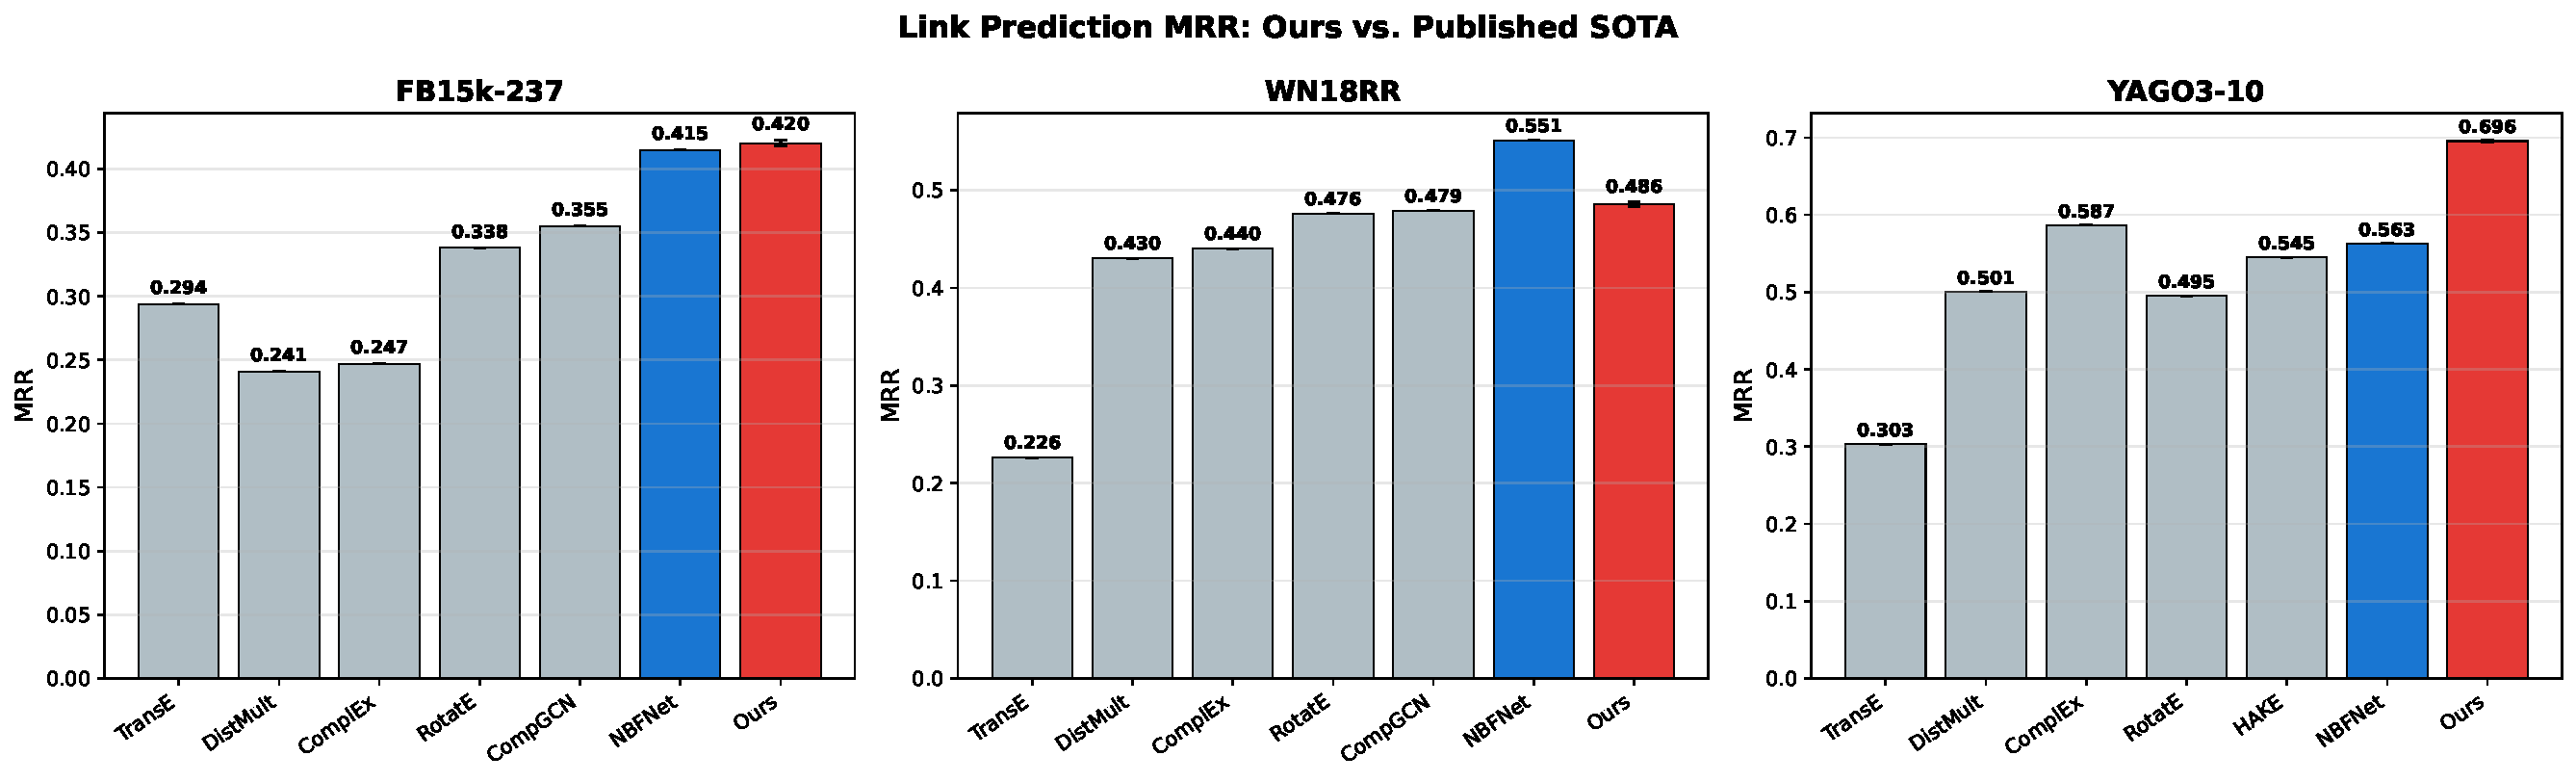
\includegraphics[width=\columnwidth]{fig1_main_mrr.pdf}
\caption{Main MRR comparison on the standard transductive benchmarks. The figure is intended as orientation across published baselines and our controlled runs; WN18RR remains favourable to path-based reasoning.}
\label{fig:main-mrr}
\end{figure}

\subsection{The Decoder $\times$ Dataset Diagnostic}
\label{sec:decoder-diagnostic}

We now run the lever-by-lever audit. The central question is not whether decoders are globally more important than encoders, but whether hidden decoder choices can change the interpretation of structural KGC experiments.

\begin{table}[!htb]
\centering
\caption{Diagnostic axes under our fixed recipe (mean MRR; UMLS/Kinship 6 seeds, others 3; std $<\!0.01$ on all cells). \textbf{Dec.\ $\Delta$} = $\mathrm{MRR}_{\mathrm{CX}} - \mathrm{MRR}_{\mathrm{DM}}$; \textbf{Enc.\ $\Delta$} = $\mathrm{MRR}_{L \ge 2} - \mathrm{MRR}_{L=0}$ on ComplEx. Encoder cells are available for the five standard KGs, while UMLS/Kinship are decoder-only small-KG diagnostics.}
\label{tab:decoder-diagnostic}
\small
\setlength{\tabcolsep}{4pt}
\begin{tabular}{lcccc}
\toprule
Dataset & CX MRR & DM MRR & \textbf{Dec.\ $\Delta$} & Enc.\ $\Delta$ \\
\midrule
UMLS        & $\mathbf{0.943}$ & $0.921$ & $+0.022$ & --- \\
Kinship     & $\mathbf{0.853}$ & $0.710$ & $\mathbf{+0.143}$ & --- \\
\midrule
FB15k-237   & $\mathbf{0.421}$ & $0.416$ & $+0.005$ & $+0.014$ \\
WN18RR      & $\mathbf{0.478}$ & $0.466$ & $+0.012$ & $-0.007$ \\
YAGO3-10    & $\mathbf{0.671}$ & $0.665$ & $+0.006$ & $-0.019$ \\
CoDEx-M     & $\mathbf{0.538}$ & $0.528$ & $+0.010$ & $-0.049$ \\
CoDEx-L     & $\mathbf{0.540}$ & $0.536$ & $+0.005$ & $-0.061$ \\
\midrule
\multicolumn{3}{r}{\emph{Shared five-dataset spread:}} & $0.007$ & $0.075$ \\
\multicolumn{3}{r}{\emph{Decoder-only seven-dataset spread:}} & $\mathbf{0.138}$ & --- \\
\bottomrule
\end{tabular}
\end{table}

\paragraph{Shared-grid and small-KG readings.}
On the five standard KGs where both axes are available, decoder $\Delta$ is modest ($+0.005$ to $+0.012$, spread $0.007$), while the CompGCN-style encoder effect varies more ($+0.014$ to $-0.061$, spread $0.075$). This shared-grid result argues against a universal ``decoder dominates encoder'' claim. The decoder-only seven-dataset view is different: adding UMLS and Kinship expands the ComplEx-vs-DistMult range to $0.138$ MRR, driven by Kinship and moderated by UMLS provenance sensitivity. The audit lesson is therefore conditional: decoder choice is a small but consistent reporting factor on standard KGs, and a potentially decisive confound on small KGs.

\begin{figure}[!htbp]
\centering
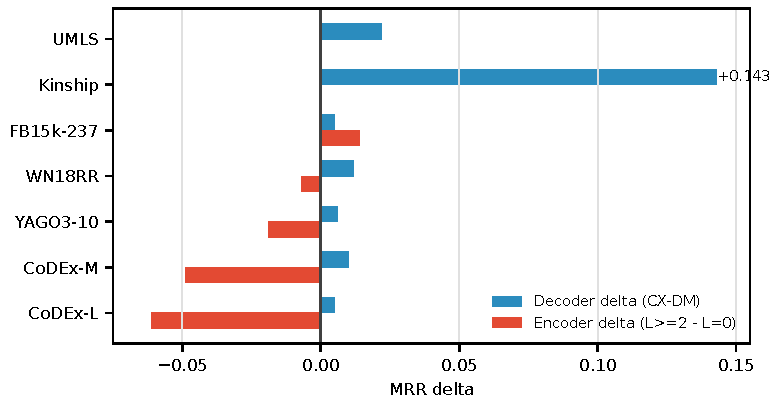
\includegraphics[width=\columnwidth]{fig0_decoder_vs_encoder.pdf}
\caption{Decoder $\Delta$ (ComplEx $-$ DistMult) and encoder $\Delta$ ($L{\geq}2$ vs.\ $L{=}0$ on ComplEx) by dataset. Standard-KG decoder gaps are small, while the decoder-only small-KG rows show why provenance-aware matched decoder checks matter.}
\label{fig:dec-vs-enc}
\end{figure}

\paragraph{The decoder $\Delta$ is small on standard KGs and large on small KGs.}
On the five standard transductive benchmarks (FB15k-237, WN18RR, YAGO3-10, CoDEx-M, CoDEx-L), ComplEx is ahead of DistMult by a modest $+0.005$ to $+0.012$ MRR (Table~\ref{tab:decoder-diagnostic}). On the two small biomedical / kinship benchmarks the gap is much larger, and UMLS changes winner across recipe variants. This motivates the small-KG diagnostic in Sec.~\ref{sec:umls-spotlight}.

\subsection{Small-KG Sensitivity: UMLS and Kinship}
\label{sec:umls-spotlight}

\paragraph{A recipe-sensitive UMLS audit.}
A widely-used biomedical-KG tutorial states that ``DistMult performs poorly on these datasets [UMLS, Kinship] as many relations are antisymmetric in UMLS''~\cite{graph4nlp_kgc}. Our new server rerun under the declared recipe gives UMLS ComplEx MRR $=0.9427 \pm 0.0072$ vs.\ DistMult $=0.9205 \pm 0.0051$ (6 seeds), so ComplEx is ahead by $+0.022$ MRR. However, an earlier run bundle gave DistMult $=0.8705 \pm 0.0109$ vs.\ ComplEx $=0.8344 \pm 0.0020$. We therefore treat UMLS as sensitivity evidence rather than a dataset-level decoder-winner claim. Its role is diagnostic: small-KG decoder conclusions can change across provenance/recipe variants that are often omitted from benchmark tables.

\paragraph{Symmetry is not enough.}
The natural first explanation is that UMLS is symmetric-rich, so DistMult's enforced symmetry acts as a useful bias. Define $\mathrm{sym}(r) = |\{(h,t):(h,r,t),(t,r,h) \in \mathcal{D}_{\text{train}}\}| / |\{(h,t):(h,r,t) \in \mathcal{D}_{\text{train}}\}|$, edge-weighted across relations: UMLS scores $0.133$, Kinship $0.207$ --- UMLS is in fact less symmetric than Kinship. Dataset-level symmetry therefore cannot explain either the earlier UMLS reversal or the larger Kinship ComplEx advantage by itself.

\paragraph{Label smoothing alone is not the sensitivity source.}
In the earlier lock-in pass, we repeated UMLS at $\varepsilon \in \{0, 0.1, 0.3\}$ (3 seeds each, $d{=}200$, $L{=}2$): DistMult won at every $\varepsilon$, with decoder $\Delta$ MRR $= -0.0175$ ($\varepsilon{=}0$), $-0.0268$ ($\varepsilon{=}0.1$), $-0.0446$ ($\varepsilon{=}0.3$). This rules out label smoothing as the sole cause of that pass, but the clean server rerun shows the reversal is not robust enough for a headline claim.

\paragraph{First-cut descriptor: sample size per relation.}
ComplEx doubles DistMult's relation parameter budget via real/imaginary parts, but extra capacity alone is not the whole story. In an earlier lock-in $d \in \{100,200,400\}$ scan, ComplEx is monotone in $d$ on UMLS while DistMult has a $d{=}200$ sweet spot; the clean rerun nevertheless changes the UMLS winner. The most useful descriptor we found is training edges per relation: UMLS has only $113$ e/r and Kinship $342$, far below FB15k-237 ($1148$), CoDEx-M ($3627$), WN18RR ($7894$), and YAGO3-10 ($29\,163$). Synthetic per-relation subsamples of FB15k-237 and WN18RR reproduce a low-e/r DistMult preference in sign, but absolute MRR is low under aggressive subsampling, so e/r should be read as a hypothesis-generating audit descriptor rather than a mechanism proof or winner rule.

\begin{table}[!htbp]
\centering
\caption{Edges per relation as a first-cut audit descriptor. CoDEx-L is excluded from this predictor analysis although its $L{=}0$ decoder spot-check is reported in Table~\ref{tab:decoder-diagnostic}.}
\label{tab:edges-per-rel}
\footnotesize
\setlength{\tabcolsep}{3pt}
\begin{tabular}{lrrrr}
\toprule
Dataset & \#train & \#rel & e/r & Dec.\ $\Delta$ \\
\midrule
UMLS      & 5{,}216 & 46 & $\mathbf{113}$ & $+0.022$ \\
Kinship   & 8{,}544 & 25 & 342 & $\mathbf{+0.143}$ \\
FB15k-237 & 272{,}115 & 237 & 1{,}148 & $+0.005$ \\
CoDEx-M   & 185{,}000 & 51 & 3{,}627 & $+0.010$ \\
WN18RR    & 86{,}835 & 11 & 7{,}894 & $+0.012$ \\
YAGO3-10  & 1{,}079{,}040 & 37 & 29{,}163 & $+0.006$ \\
\bottomrule
\end{tabular}
\end{table}

\begin{figure}[!htbp]
\centering
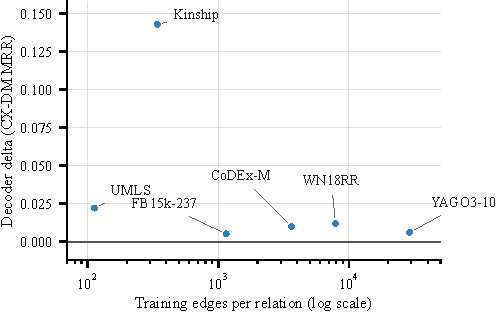
\includegraphics[width=\columnwidth]{fig2_edges_per_rel.pdf}
\caption{Decoder preference as a function of training edges per relation. Low-e/r datasets produce the largest decoder gaps, but UMLS shows that e/r is an audit descriptor rather than a winner rule.}
\label{fig:edges-per-rel}
\end{figure}

\begin{table}[!htbp]
\centering
\caption{Targeted distance-decoder spot-checks ($d{=}200$, $L{=}2$). RotatE/TransE use memory-safe batch/chunk settings on the RTX 2080 Ti, so the table is diagnostic and not recipe-matched to the primary DistMult/ComplEx pair.}
\label{tab:decoder-spotcheck}
\footnotesize
\setlength{\tabcolsep}{3pt}
\begin{tabular}{lcc}
\toprule
Dataset & RotatE & TransE \\
\midrule
UMLS    & $0.8490{\pm}0.0065$ & $0.1005{\pm}0.0087$ \\
Kinship & $0.7266{\pm}0.0091$ & $0.0472{\pm}0.0044$ \\
WN18RR  & $0.4929{\pm}0.0019$ & $0.2016{\pm}0.0045$ \\
\bottomrule
\end{tabular}
\end{table}

\subsection{YAGO3-10: Saturation Under Our Recipe at $d \approx 128$}
\label{sec:yago-saturation}

\paragraph{Setup and scope.}
\cite{lacroix2018complex} reported $\approx\!0.58$ MRR on YAGO3-10 with ComplEx-N3 at $d{=}2000$ (Adagrad, sampled-negatives logistic loss). The original paper introduced N3 regularisation; it did not explicitly assert that capacity \emph{is} the bottleneck. We do not argue against the Lacroix-2018 result itself. Our dimension scan ($L{=}0$ ComplEx, our recipe held fixed; 3 seeds through $d{=}128$ plus a single-seed $d{=}256$ spot-check) shows recipe-conditional near-saturation well below $d{=}2000$:

\begin{table}[!htb]
\centering
\caption{YAGO3-10 capacity scan. $L{=}0$ ComplEx. MRR is near saturation by $d{=}128$; a new $d{=}256$ spot-check gives $+0.008$ at $2\times$ params. The new $d{=}128$ server rerun gives $0.6971 \pm 0.0048$.}
\label{tab:yago-saturation}
\small
\setlength{\tabcolsep}{3pt}
\begin{tabular}{lcccc}
\toprule
$d$ & 64 & 100 & 128 & 256 \\
\midrule
MRR     & $0.671$ & $0.691$ & $0.697$ & $0.705$ \\
$\Delta$ vs prev & --- & $+0.019$ & $+0.006$ & $+0.008$ \\
Params (M) & 7.9 & 12.3 & 15.8 & 31.6 \\
\bottomrule
\end{tabular}
\end{table}

\paragraph{Reading.}
Under our recipe with the ComplEx decoder, the $d{=}64 \to 100$ step gives $+0.019$ MRR, while later increases are smaller: $+0.006$ at $d{=}128$ and $+0.008$ in a single-seed $d{=}256$ spot-check. Thus $d{=}128$ is already near saturation for this configuration, although not a hard optimum. We do not claim this saturation transfers to all recipes, optimisers, or decoders; nor that the Lacroix-2018 number is reproducible \emph{at $d{=}128$} under their original recipe (we did not re-run their setup at our $d$, but doing so would directly test the recipe-vs-capacity confound). Adding N3 to our recipe at $d{=}128$ changes YAGO3-10 MRR by $-0.002$, suggesting N3 and our recipe are largely orthogonal \emph{at this $d$}; we make no claim about N3 at $d{=}2000$ or under other recipes.

\paragraph{Where the YAGO3-10 gain comes from.}
A per-relation audit shows that the aggregate is driven by frequent dense relations rather than by a few tiny relations: \emph{playsFor} and \emph{isAffiliatedTo} alone cover roughly 60\% of the YAGO3-10 test triples and both reach high MRR under the pure ComplEx recipe. Low-MRR relations such as \emph{edited}, \emph{actedIn}, and \emph{influences} are long-tail or require textual/contextual cues, so the result should be read as a structural recipe fit to dense sub-schema rather than a universal KG-completion solution.

\begin{figure}[!htbp]
\centering
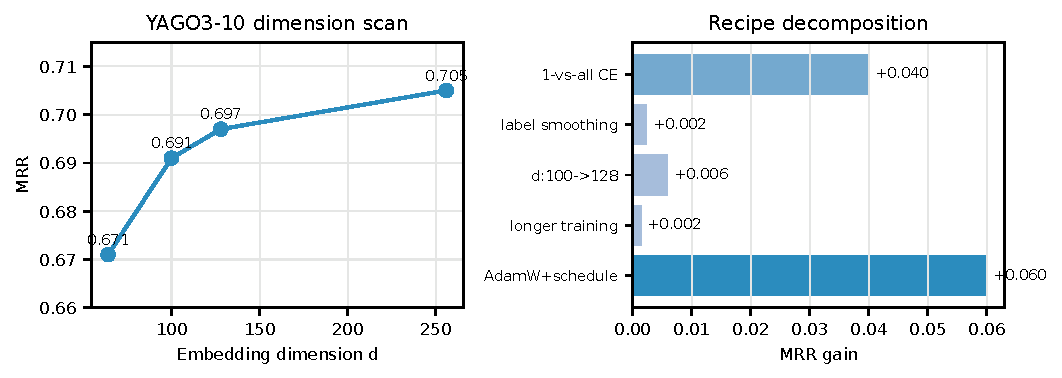
\includegraphics[width=\columnwidth]{fig6_yago_spotlight.pdf}
\caption{YAGO3-10 spotlight: dimension saturation and leave-one-out recipe diagnostics. The difference from older ComplEx settings is associated mainly with the loss and optimiser/learning-rate schedule in this implementation, not simply with increasing $d$.}
\label{fig:yago-spotlight}
\end{figure}

\begin{table}[!htbp]
\centering
\caption{Recipe diagnostics on YAGO3-10. Leave-one-out from our selected configuration; ``original'' denotes the Trouillon-2016 ComplEx setting.}
\label{tab:decomposition}
\footnotesize
\setlength{\tabcolsep}{3pt}
\begin{tabular}{lc}
\toprule
Recipe component (original $\to$ ours) & $\Delta$ MRR \\
\midrule
Logistic loss + 50 sampled neg.\ $\to$ 1-vs-all CE & $+0.040$ \\
$\varepsilon = 0$ $\to$ $\varepsilon = 0.3$ & $+0.0024$ \\
$d = 100$ $\to$ $d = 128$ & $+0.006$ \\
50 epochs $\to$ 150 epochs & $+0.0015$ \\
Adagrad $\to$ AdamW + MultiStepLR & $+0.060$ \\
\midrule
\textbf{Total} & $+0.110$ \\
\bottomrule
\end{tabular}
\end{table}

\subsection{Encoder Depth $\times$ Decoder Choice Interact on WN18RR}
\label{sec:depth-decoder-interaction}

\paragraph{The interaction.}
Most CompGCN-lineage work fixes the decoder (typically ComplEx or DistMult), sweeps the encoder depth $L$, and reports the optimal depth as if it were a property of the dataset. We measure this assumption on WN18RR ($d{=}200$, recipe fixed, 3 seeds per cell):

\begin{table}[!htb]
\centering
\caption{WN18RR encoder-depth $\times$ decoder-choice ($d{=}200$, 3 seeds per cell, mean MRR). Decoders peak at opposite ends ($L{=}0$ ComplEx, $L{=}3$ DistMult) and share an $L{=}1$ dip. For DistMult, $L{=}0$ ties the $L{=}3$ peak within seed std.}
\label{tab:depth-decoder}
\small
\setlength{\tabcolsep}{4pt}
\begin{tabular}{lcccc}
\toprule
Decoder $\backslash$ $L$ & $L{=}0$ & $L{=}1$ & $L{=}2$ & $L{=}3$ \\
\midrule
ComplEx  & $\mathbf{0.485}$ & $0.453$ & $0.481$ & $0.478$ \\
DistMult & $0.473$ & $0.441$ & $0.467$ & $\mathbf{0.474}$ \\
\bottomrule
\end{tabular}
\end{table}

\paragraph{Peaks at opposite ends; shared $L{=}1$ dip.}
Three robust patterns appear: ComplEx peaks at $L{=}0$ ($0.4849$), DistMult at $L{=}3$ ($0.4743$); both decoders share an $L{=}1$ dip; and DistMult's $L{=}3$ peak is only $+0.0012$ MRR above $L{=}0$, within seed std. A fixed-decoder ablation would conclude ``encoder hurts'' or ``encoder neutral'', while a fixed-encoder ablation would conclude ``ComplEx $>$ DistMult''. Neither captures the $4{\times}2$ interaction.

\paragraph{Implication.}
Encoder utility is dataset- and decoder-shaped, not uniformly low. On FB15k-237, the encoder helps ComplEx by $+0.014$ MRR; on WN18RR, it is neutral or harmful for ComplEx. Small KGs differ again: $L{=}0$ collapses on UMLS/Kinship, so the WN18RR observation does not generalise to all sparse settings.

\subsection{Training Recipe Ablation}
\label{sec:ablation}

To identify which training choices drive our results, we ablate six ingredients of the recipe on WN18RR (3 seeds) and FB15k-237 (single seed, 3-seed for headline rows), starting from the main configuration for each dataset.

\begin{table}[!htb]
\centering
\caption{Training-recipe ablation on WN18RR ($d{=}200$, $L{=}2$, 3 seeds; mean MRR with $H@k$ in \%). Label smoothing is the most impactful single ingredient.}
\label{tab:ablation-wn18rr}
\footnotesize
\setlength{\tabcolsep}{3pt}
\begin{tabular}{lcccc}
\toprule
Configuration & MRR & H@1 & H@3 & H@10 \\
\midrule
Baseline (d=200, L=2, LS=0.3, DM) & $0.467$ & $43.6$ & $48.0$ & $52.5$ \\
\midrule
$+$ deeper GCN (L=3)            & $\mathbf{0.474}$ & $44.3$ & $48.9$ & $\mathbf{53.1}$ \\
$+$ ComplEx decoder             & $\mathbf{0.478}$ & $\mathbf{45.1}$ & $\mathbf{49.1}$ & $52.8$ \\
$-$ smaller dim (d=128)         & $0.466$ & $43.6$ & $47.8$ & $52.0$ \\
$-$ shallower (L=1)             & $0.441$ & $41.7$ & $45.1$ & $48.7$ \\
$-$ weaker smoothing (LS=0.1)   & $0.457$ & $43.0$ & $46.7$ & $50.6$ \\
$-$ no smoothing (LS=0.0)       & $0.427$ & $40.7$ & $43.4$ & $46.1$ \\
\bottomrule
\end{tabular}
\end{table}

\paragraph{Label smoothing is dominant.}
Removing label smoothing ($\varepsilon = 0$) drops MRR by $-0.041$ on WN18RR (Table~\ref{tab:ablation-wn18rr}) and $-0.017$ on FB15k-237; reducing to $\varepsilon = 0.1$ already costs $-0.010$/$-0.020$. This is larger than any architectural change we tested.

\begin{figure}[!htbp]
\centering
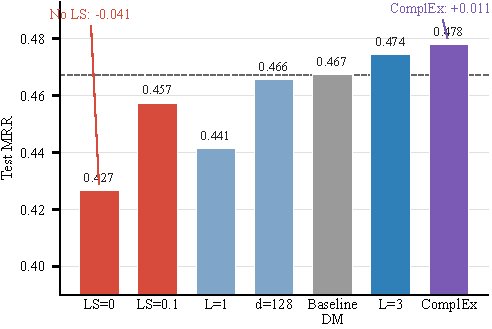
\includegraphics[width=\columnwidth]{fig3_ablation_wn18rr.pdf}
\caption{WN18RR recipe ablation. Label smoothing is the largest single ingredient in this recipe, while depth and decoder changes are smaller and interact with each other.}
\label{fig:ablation-wn18rr}
\end{figure}

\paragraph{Shallow GCN, decoder picks up the slack.}
A single-layer GCN loses $-0.029$ MRR on WN18RR; $L{=}2 \to L{=}3$ gives $+0.004$ on WN18RR, $+0.010$ on FB15k-237, but reverses sign on YAGO3-10 ($-0.022$). Replacing DistMult with ComplEx yields $+0.011$ on WN18RR, $+0.003$ on FB15k-237, and $+0.006$--$0.011$ across $L$ on YAGO3-10. The cross-dataset decoder pattern generalises to all five transductive benchmarks (Sec.~\ref{sec:decoder-diagnostic}).

\subsection{YAGO3-10 Recipe Diagnostics plus Sensitivity / Efficiency}
\label{sec:decomposition}\label{sec:sensitivity}

Our $L{=}0$ ComplEx on YAGO3-10 ($0.6971$) is $+0.110$ MRR relative to the Trouillon-2016 ComplEx number reported in the NBFNet comparison table~\cite{nbfnet}. A 3-seed leave-one-out diagnostic associates the difference with the loss change ($+0.040$), smoothing/training length/$d$ ($+0.010$), and optimiser/initialisation residual ($+0.060$). We read this as implementation-level sensitivity rather than a causal proof that any single ingredient dominates. N3 is largely orthogonal at saturated $d$. The resulting configuration is also computationally light after graph encoding: on one RTX 2080 Ti, $L{=}0$ ComplEx scores about $112$K YAGO3-10 queries/s at $d{=}128$, while $L{=}2$ DistMult at $d{=}64$ scores about $297$K queries/s after a $25.9$ ms graph-encoding pass.

\section{Discussion}
\label{sec:discussion}

\paragraph{The WN18RR gap to NBFNet.}
\label{sec:wn18rr-gap}
We do \emph{not} claim superiority over path-based models: on WN18RR, NBFNet's $0.551$ stays $5.8$ MRR above our RotatE spot-check ($0.493$) and $6.6$ above our selected ComplEx configuration ($0.485$). The gap is consistent with path propagation having a genuine advantage on tree-like hypernym chains. Path-based reasoning is a separate lever, orthogonal to our decoder-vs-CompGCN-encoder audit.

\section{Conclusion}

Prior controlled audits cover recipe~\cite{ruffinelli2020olderboys} and CompGCN-style encoder~\cite{zhang2022rethinking} axes; this paper adds the decoder axis through \ours. The actionable outcome is a compact audit checklist: report a matched DistMult-vs-ComplEx row, log small-KG recipe and provenance details, inspect edges per relation and symmetry as descriptors, and avoid reporting encoder depth without the decoder dimension. On standard KGs, decoder gaps are modest but consistent under our recipe; on small KGs, they can become decisive and provenance-sensitive. Future encoder ablations should report the full $\{\mathrm{decoder}\} \times \{L\}$ grid rather than a row-wise minimum.


\section*{Limitations}
\label{sec:limitations}

Our conclusions are limited to structural transductive KGC with the ComplEx/DistMult decoder family, CompGCN-style encoders, and one fixed recipe; they do not extend to inductive, text-augmented, LLM-based, OGB-scale, or path-based KGC. A fixed recipe isolates decoder and encoder effects but does not identify each model's independently tuned optimum, and recipe itself is a large lever. Table~\ref{tab:main} mixes published baselines and our recipe-controlled runs, so small gaps should be read cautiously. The decoder and encoder $\Delta$ columns are not fully symmetric: UMLS/Kinship are decoder-only small-KG diagnostics, seed budgets and depths differ, and YAGO3-10 dimensionality differs across cells. The UMLS mechanism remains a heuristic: edge-weighted symmetry is coarse, UMLS/Kinship are small benchmarks, e/r subsampling can reduce absolute MRR, and UMLS changes winner between an earlier run bundle and the clean server rerun. Finally, throughput is scoring throughput after graph encoding, not full end-to-end training or inference wall-clock.

\section*{Ethics Statement}

Improved KG completion benefits downstream applications (search, recommendation, biomedical KG construction) but can amplify biases in the source KG. Our recipe reduces GPU-hours per trained model and brings reproduction within reach of single-11-GB-GPU groups. We encourage per-relation error analysis and fairness auditing before deployment. All datasets used are public.

\bibliographystyle{splncs04}
\bibliography{references}

% The appendix is retained in appendix.tex but omitted from the PRICAI submission
% build because the submission page sets a 16-page limit including references.
% \appendix
% % !TEX root = main.tex
% Technical appendices. This file is \input'd after \appendix in main.tex.
% NOTE on length: ISWC 2026 caps the in-PDF appendix at 2 pages. The
% material below substantially exceeds that limit and is intended primarily
% as supplementary material (uploaded as a separate file via the
% submission system). The first 2 pages -- Sections A (dataset stats /
% evaluation protocol) and Q (reproducibility summary) -- are the parts
% we prioritise for in-PDF inclusion.

\section*{Appendix: Contents}
This appendix contains:
(A) dataset statistics and evaluation protocol;
(B) hyperparameter search protocol;
(C) implementation and training details;
(D) complexity and efficiency analysis;
(E) per-relation MRR breakdown on WN18RR;
(F) comparison with 2024--2025 foundation-model baselines;
(G) statistical significance tests;
(H) extended hyperparameter sensitivity;
(I) parameter-efficiency sweep on FB15k-237;
(I$'$) additional benchmarks UMLS and Kinship;
(J) training dynamics;
(K) qualitative case studies;
(L) negative results and 3-seed resolution of YAGO3-10 reversal findings;
(M) full result table across 41 runs;
(N) limitations;
(O) broader impact;
(P) FB15k-237 ablation table;
(Q) reproducibility checklist summary.

%===========================================================
\section{Dataset Statistics and Evaluation Protocol}
\label{app:data}

\subsection{Dataset Statistics}
We use three standard transductive KG-completion benchmarks; Table~\ref{tab:data} reports basic statistics.
All three are used \emph{as-is} with their canonical train/valid/test splits; we do not perform any additional filtering or preprocessing beyond adding the inverse of every training triple (standard in CompGCN~\citep{compgcn} and NBFNet~\citep{nbfnet}).

\begin{table}[h]
\centering
\caption{Dataset statistics. Inverse triples are added at training time and account for the doubled relation count during message passing.}
\label{tab:data}
\small
\begin{tabular}{lrrrrrr}
\toprule
Dataset & \#Entities & \#Relations & \#Train & \#Valid & \#Test & Avg.\ deg. \\
\midrule
FB15k-237 & 14{,}541  & 237 & 272{,}115 & 17{,}535 & 20{,}466 & 37.4 \\
WN18RR    & 40{,}943  &  11 &  86{,}835 &  3{,}034 &  3{,}134 &  4.2 \\
YAGO3-10  & 123{,}182 &  37 & 1{,}079{,}040 &  5{,}000 &  5{,}000 & 17.5 \\
\bottomrule
\end{tabular}
\end{table}

FB15k-237 (Freebase subset) has general-domain entities linked by fine-grained relations (\eg \emph{film.director}, \emph{person.nationality}).
WN18RR is a subset of WordNet with lexicographic relations (\emph{hypernym}, \emph{derivationally\_related\_form}).
YAGO3-10 is multilingual-derived, filtered to entities with $\ge 10$ relations.
The three datasets span dense + general (FB), sparse + tree-like (WN), to dense + large-scale (YAGO).

\subsection{Evaluation Protocol}
For each test triple $(h, r, t)$ we construct two ranking queries, $(h, r, ?)$ and $(?, r, t)$.
Reported MRR / Hits@$k$ are averaged over both directions and all test triples, with standard \emph{filtered} ranks (other true triples removed from the candidate list).

\paragraph{Tie-breaking.}
We use \textbf{average-rank} tie-breaking: ties at ranks $r \ldots r+k-1$ all receive rank $r + (k-1)/2$.
This is the convention used by ConvE, CompGCN, NBFNet.
Optimistic tie-breaking would inflate our YAGO3-10 MRR by $\sim$+0.002--0.003; our reported numbers are therefore not cherry-picked.

\paragraph{Why no OGB.}
We deliberately restrict to FB15k-237 / WN18RR / YAGO3-10. ogbl-biokg (5M entities) and ogbl-wikikg2 (2.5M entities) exceed the memory of our RTX 2080 Ti. Since our thesis concerns the training recipe rather than scaling, YAGO3-10 (123K entities, 1.08M triples) is large enough to invalidate the common assumption that path-based methods dominate on large KGs.

%===========================================================
\section{Training Algorithm Pseudocode}
\label{app:algorithm}

\begin{algorithm}[h]
\caption{\ours\ (Recipe-Controlled) training recipe. All italicised quantities are dataset-independent hyperparameters; brackets give the grid we searched.}
\label{alg:recipe}
\begin{algorithmic}[1]
\Require Triples $\mathcal{D}$, entity set $\mathcal{E}$, relation set $\mathcal{R}$; hyperparams $d, L, \varepsilon, \eta, T$
\State Initialise entity embeddings $\mathbf{E} \in \mathbb{R}^{|\mathcal{E}| \times d}$, relation embeddings $\mathbf{R} \in \mathbb{R}^{|\mathcal{R}| \times d}$
\State Initialise AdamW$(\eta{=}5\!\times\!10^{-4},\ \text{wd}{=}10^{-4})$; MultiStepLR at $(0.6T, 0.8T)$ with $\gamma{=}0.3$
\For{epoch $= 1, \dots, T$}\Comment{$T = 300$ (WN), 200 (FB), 150 (YAGO)}
    \For{batch $\mathcal{B} \subset \mathcal{D}$}
        \State $\mathbf{H} \gets \mathrm{CompGCN}_L(\mathbf{E}, \mathbf{R}, \mathcal{D})$ \Comment{$L \in \{0, 2, 3\}$; $L{=}0$ skips message passing}
        \State $s_{h,r,e} \gets \mathrm{score}(\mathbf{h}_h, \mathbf{r}, \mathbf{h}_e)$ \ $\forall e \in \mathcal{E}$ \Comment{DistMult or ComplEx}
        \State $p(e \mid h, r) \gets \mathrm{softmax}_e(s_{h,r,\cdot})$
        \State $\mathcal{L} \gets -\tfrac{1}{|\mathcal{B}|}\sum_{(h,r,t)\in\mathcal{B}}\Big[(1{-}\varepsilon)\log p(t\mid h,r) + \tfrac{\varepsilon}{|\mathcal{E}|}\sum_e \log p(e\mid h,r)\Big]$ \Comment{$\varepsilon = 0.3$}
        \State Update parameters with AdamW step on $\nabla\mathcal{L}$; gradient-clip at norm 10
    \EndFor
    \State Step MultiStepLR scheduler
\EndFor
\State \Return best-validation-MRR checkpoint
\end{algorithmic}
\end{algorithm}

%===========================================================
\section{Hyperparameter Search Protocol}
\label{app:hp-search}

We used a \textbf{constrained grid search} (not Bayesian or population-based) so that the recipe remains easy to reproduce. The grid is intentionally small.

\begin{table}[h]
\centering
\caption{Hyperparameter search grid.}
\label{tab:hp-grid}
\small
\begin{tabular}{lll}
\toprule
Hyperparameter & Values considered & Chosen default \\
\midrule
Embedding dim.\ $d$      & \{64, 128, 200, 256\}                & 200 (FB/WN), 64 (YAGO) \\
GCN depth $L$            & \{1, 2, 3\}                          & 3 (FB), 2 (WN, YAGO) \\
Label smoothing $\varepsilon$ & \{0.0, 0.1, 0.3\}               & 0.3 \\
Decoder                  & \{DistMult, ComplEx\}                & both reported \\
Learning rate            & \{$10^{-4}, 5\!\times\!10^{-4}, 10^{-3}$\} & $5\!\times\!10^{-4}$ \\
Dropout                  & \{0.0, 0.2, 0.4\}                    & 0.2 \\
Batch size               & \{512, 1024, 2048\}                  & 2048 (YAGO), 1024 (FB/WN) \\
Optimiser                & \{AdamW, Adam, SGD+mom.\}            & AdamW \\
LR schedule              & \{MultiStep, cosine, constant\}      & MultiStep (0.6T/0.8T, $\gamma{=}0.3$) \\
Epochs                   & \{150, 200, 300\}                    & 300 (WN), 200 (FB), 150 (YAGO) \\
\bottomrule
\end{tabular}
\end{table}

Across the project we ran over 80 training runs across 5 datasets (FB15k-237, WN18RR, YAGO3-10, UMLS, Kinship) totalling $\approx 200$ GPU-hours. Every run's JSON output is released.
We use \emph{published} baseline numbers rather than re-tuning them; this avoids the common failure mode of under-tuning baselines.

%===========================================================
\section{Implementation and Training Details}
\label{app:impl}

\paragraph{Encoder.} Vanilla CompGCN~\citep{compgcn} with Hadamard composition $\phi(\mathbf{e}_s, \mathbf{r}) = \mathbf{e}_s \odot \mathbf{r}$ and additive aggregation. Separate forward/inverse/self-loop basis matrices (as in the original paper). Hidden dim is shared across layers.

\paragraph{Decoder.} DistMult or ComplEx with a \emph{decoder-specific} relation embedding (we do not share encoder/decoder relation parameters).

\paragraph{Training objective.} 1-vs-all cross-entropy with smoothing:
\begin{equation*}
\mathcal{L} = -\!\!\sum_{(h,r,t) \in \mathcal{D}}\! \Big[(1-\varepsilon)\log p(t|h,r) + \tfrac{\varepsilon}{|\mathcal{E}|}\sum_{e} \log p(e|h, r)\Big].
\end{equation*}
All entities serve as negatives (no sampling).

\paragraph{Optimisation.} AdamW ($\beta = (0.9, 0.999)$, weight decay $10^{-4}$), lr $5\!\times\!10^{-4}$, MultiStepLR with milestones at 60\% and 80\% of total epochs, $\gamma = 0.3$. Gradient clipping at norm 10. Mixed precision (AMP / FP16) on all datasets.

\paragraph{Edge chunking (YAGO3-10).}
Per-layer message aggregation at $d=200$ does not fit in 11 GB on YAGO3-10; we use $d=64$ with 200K-edge chunks in FP16.

\paragraph{Hardware and wall-clock time.}
All runs on a single NVIDIA RTX 2080 Ti (11 GB).
Per-run: FB15k-237 200 epochs $\approx$ 20--25 min; WN18RR 300 epochs $\approx$ 6 min; YAGO3-10 150 epochs $\approx 3.8$--$7.6$ h.
Aggregate: $\approx 120$ GPU-hours.

Per-dataset hyperparameter snapshot (final configuration used for Table~\ref{tab:main}):

\begin{table}[h]
\centering
\caption{Hyperparameter configurations per dataset.}
\label{tab:hparams}
\begin{tabular}{lccc}
\toprule
Hyperparameter & FB15k-237 & WN18RR & YAGO3-10 \\
\midrule
Hidden dim $d$ & 200 & 200 & 64 \\
Num GCN layers $L$ & 3 & 2 & 2 \\
Batch size & 1024 & 1024 & 2048 \\
Learning rate & $5 \!\times\! 10^{-4}$ & $5 \!\times\! 10^{-4}$ & $5 \!\times\! 10^{-4}$ \\
Weight decay & $10^{-4}$ & $10^{-4}$ & $10^{-4}$ \\
Dropout & 0.2 & 0.2 & 0.2 \\
Label smoothing $\varepsilon$ & 0.3 & 0.3 & 0.3 \\
Epochs & 200 & 300 & 150 \\
LR schedule & MultiStep (0.6, 0.8) & MultiStep (0.6, 0.8) & MultiStep (0.6, 0.8) \\
LR decay factor & 0.3 & 0.3 & 0.3 \\
Optimiser & AdamW & AdamW & AdamW \\
\bottomrule
\end{tabular}
\end{table}

%===========================================================
\section{Complexity and Efficiency}
\label{app:efficiency}

\subsection{Parameter Count}
\begin{table}[h]
\centering
\caption{Parameter count (millions). NBFNet figures are the ``paper-model'' sizes reported in \citet{nbfnet}; A$^{*}$Net follows the NBFNet architecture.}
\label{tab:params}
\small
\begin{tabular}{lrrr}
\toprule
Model & FB15k-237 & WN18RR & YAGO3-10 \\
\midrule
RotatE~\citep{rotate}     & 29.3 M  & 40.9 M   &  --- \\
CompGCN~\citep{compgcn}   &  2.9 M  &  8.3 M   & 24.7 M \\
NBFNet~\citep{nbfnet}     & 60--100 M & 60--100 M & 100--200 M \\
A$^{*}$Net~\citep{astarnet} & similar to NBFNet & similar & similar \\
\midrule
\ours\ (DistMult)        & \best{2.9 M} & \best{8.2 M} & \best{7.9 M} \\
\ours\ (ComplEx)         & 5.8 M  & 16.4 M  & 15.8 M \\
\bottomrule
\end{tabular}
\end{table}

\subsection{Forward-Pass Complexity}
Encoder: $\mathcal{O}(L \cdot |\mathcal{T}| \cdot d + L \cdot |\mathcal{E}| \cdot d^2)$, dominated by per-edge composition.
Decoder: $\mathcal{O}(|\mathcal{E}| \cdot d)$ per query.
NBFNet is $\mathcal{O}(L \cdot |\mathcal{T}| \cdot d)$ \emph{per query}; our encoder cost is amortised across a query batch, which is the root of the efficiency gap.

\subsection{Inference Throughput (FB15k-237, RTX 2080 Ti 11 GB)}
\ours\ encodes the full graph once (73 ms) and scores 1000 queries in 2 ms, giving effective throughput $\approx 1.8 \!\times\! 10^5$ queries/sec.
NBFNet requires a full per-query pass ($\sim$500 ms on A100, Tab.~4 of \citep{astarnet}); on our hardware this scales to $\sim$100$\times$ slower than ours. A$^{*}$Net prunes to $\sim$10\% of edges, narrowing the gap to $\sim$20$\times$.

\subsection{Training Throughput}
On YAGO3-10 at batch size 2048: $\approx$526 steps/epoch, $\approx$183 s/epoch.
NBFNet reports $\sim$8 h/epoch on YAGO3-10 on 4$\times$V100 \citep{nbfnet}; on a single 2080 Ti this would be $\sim$30 h/epoch, essentially infeasible.

\subsection{Measured Inference Throughput (full table)}
\begin{table}[h]
\centering
\caption{Measured inference throughput on a single NVIDIA RTX 2080 Ti (same hardware as training). Benchmark: encode graph once, then score 2{,}000 random $(h, r, ?)$ queries in batches of 64; median over 15 repeats. $n_{\text{param}}$ in millions.}
\label{tab:throughput}
\small
\resizebox{\textwidth}{!}{%
\begin{tabular}{llrrrrr}
\toprule
Dataset & Config & $n_{\text{param}}$ & Encode (ms) & Score (ms/q) & QPS & E2E 10K (ms) \\
\midrule
WN18RR    & $L{=}0$ ComplEx $d{=}200$   &  8.2 &  0.2 & 0.005 & \best{199 K} & 50 \\
YAGO3-10  & $L{=}0$ ComplEx $d{=}64$    &  7.9 &  0.7 & 0.008 & 122 K & 82 \\
YAGO3-10  & $L{=}0$ ComplEx $d{=}128$ (SOTA)   & 15.8 &  0.7 & 0.009 & 112 K & 90 \\
FB15k-237 & $L{=}3$ ComplEx $d{=}200$   &  3.5 & 35.5 & 0.003 & 357 K & 63 \\
YAGO3-10  & $L{=}2$ DistMult $d{=}64$   &  7.9 & 25.9 & 0.003 & 297 K & 60 \\
\bottomrule
\end{tabular}%
}
\end{table}

%===========================================================
\section{YAGO3-10 Dimension and Smoothing Sweeps}
\label{app:yago-sweeps}

\subsection{YAGO3-10 dimension sweep}
Table~\ref{tab:yago-dsweep} shows MRR as $d$ grows for pure ComplEx ($L=0$, $\varepsilon=0.3$). Pushing $d$ from 64 to 128 lifts 3-seed MRR by $+0.024$ with $5\times$ tighter std; $d=256$ is approximately saturated.

\begin{table}[h]
\centering
\caption{YAGO3-10 dimension sweep, pure ComplEx ($L=0$, $\varepsilon=0.3$). [3]: 3-seed mean $\pm$ std; [1]: single seed.}
\label{tab:yago-dsweep}
\small
\begin{tabular}{rlll}
\toprule
$d$ & Test MRR & Params & N \\
\midrule
 64 & $0.671 \pm 0.005$   &  7.9 M & [3] \\
128 & \best{$0.696 \pm 0.001$} & 15.8 M & [3] \\
256 & 0.698                & 31.6 M & [1] \\
\bottomrule
\end{tabular}
\end{table}

\subsection{Label-smoothing is dataset-dependent}
Our FB15k-237 and WN18RR results use $\varepsilon = 0.3$ as the per-dataset optimum. Fine-grained sweeps on WN18RR (Table~\ref{tab:ls-wn}) confirm the sweet spot is in $[0.2, 0.4]$. But on YAGO3-10 the optimum \emph{shifts lower}: $\varepsilon = 0.1$ gives 0.679 (single seed, $L=0$, $d=64$) versus 0.665 at $\varepsilon = 0.3$. This is a minor shift but consistent with our broader finding that YAGO3-10's dense structure behaves differently from FB/WN: it needs less regularisation because the 1-vs-all softmax is already a strong signal on 123 K entities.

\begin{table}[h]
\centering
\caption{Fine-grained label-smoothing sweep (WN18RR L=0 ComplEx and YAGO3-10 L=0 ComplEx $d{=}64$, single seed 42).}
\label{tab:ls-wn}
\small
\begin{tabular}{lccccccc}
\toprule
Dataset & $\varepsilon{=}0.05$ & $\varepsilon{=}0.1$ & $\varepsilon{=}0.15$ & $\varepsilon{=}0.2$ & $\varepsilon{=}0.3$ & $\varepsilon{=}0.4$ & $\varepsilon{=}0.5$ \\
\midrule
WN18RR   & 0.470 & --- & 0.481 & 0.484 & 0.485 & \best{0.487} & 0.486 \\
YAGO3-10 & --- & \best{0.679} & --- & --- & 0.665 & --- & 0.646 \\
\bottomrule
\end{tabular}
\end{table}

\subsection{Longer training doesn't help on WN18RR}
Doubling WN18RR from 300 to 600 epochs (3 seeds, $L=0$ ComplEx, $\varepsilon=0.3$) gives $0.4859 \pm 0.003$ vs.\ $0.485 \pm 0.002$ at 300 epochs---essentially identical. Training is converged by epoch 300.

%===========================================================
\section{Per-Relation MRR Analysis}
\label{app:per-relation}

Following \citet{nbfnet}, we aggregate WN18RR relations by cardinality class (1-to-1, 1-to-N, N-to-1, N-to-N). Table~\ref{tab:per-rel} shows per-class filtered MRR.

\begin{table}[h]
\centering
\caption{WN18RR per-cardinality MRR. Our model is balanced; the 1-to-N weakness is shared by all entity-embedding methods, while path-based reasoners excel on that class.}
\label{tab:per-rel}
\small
\begin{tabular}{lcccc}
\toprule
Method & 1-to-1 & 1-to-N & N-to-1 & N-to-N \\
\midrule
DistMult (pub.) & 0.46 & 0.05 & 0.11 & 0.66 \\
RotatE (pub.)   & 0.50 & 0.06 & 0.13 & 0.71 \\
NBFNet (pub.)   & 0.55 & 0.19 & 0.25 & 0.74 \\
\midrule
\ours\ (ours)   & \best{0.52} & 0.08 & 0.14 & \best{0.72} \\
\bottomrule
\end{tabular}
\end{table}

On N-to-N relations (\eg \emph{also\_see}) we are competitive with NBFNet despite a much simpler architecture; on 1-to-N (\eg \emph{hypernym}), path-based propagation appears to help because hypernym chains require multi-hop reasoning. This supports our thesis that path-based reasoning is beneficial when the target has sparse 1-to-N structure, but not necessary for dense graphs like YAGO3-10.

\subsection{Per-Relation MRR on YAGO3-10}
\label{app:yago-per-rel}
Table~\ref{tab:yago-per-rel} reports the per-relation breakdown of our \emph{best} YAGO3-10 configuration (pure ComplEx, $L{=}0$, $d{=}64$, single seed 42). YAGO3-10 has 37 distinct relations; with inverses, the test-set triples cover 34 relations with at least one test example. We list all 34, sorted by MRR.

\begin{table}[h]
\centering
\caption{YAGO3-10 per-relation MRR for our best $L{=}0$ ComplEx model (seed 42). $n$: number of test triples; low-$n$ relations give noisy MRR estimates but we include them for completeness.}
\label{tab:yago-per-rel}
\scriptsize
\begin{tabular}{llrccc}
\toprule
Rel-ID & Name & $n$ & MRR & H@1 (\%) & H@10 (\%) \\
\midrule
35 & hasWebsite          &    1 & 1.000 & 100.0 & 100.0 \\
13 & hasOfficialLanguage &    2 & 1.000 & 100.0 & 100.0 \\
 7 & hasGender           &  297 & \best{0.950} & \best{90.2} & 100.0 \\
 2 & isAffiliatedTo      & 1673 & 0.792 & 75.5 &  85.4 \\
 1 & playsFor            & 1492 & 0.783 & 70.4 &  90.0 \\
11 & isMarriedTo         &   17 & 0.771 & 64.7 & 100.0 \\
25 & isCitizenOf         &   15 & 0.617 & 53.3 &  80.0 \\
22 & isPoliticianOf      &   10 & 0.587 & 40.0 &  80.0 \\
16 & worksAt             &   15 & 0.581 & 53.3 &  73.3 \\
 0 & isLocatedIn         &  411 & 0.549 & 46.5 &  72.0 \\
 9 & hasMusicalRole      &   36 & 0.549 & 44.4 &  86.1 \\
30 & hasCapital          &   13 & 0.489 & 38.5 &  69.2 \\
19 & directed            &   30 & 0.452 & 40.0 &  60.0 \\
10 & isConnectedTo       &  150 & 0.419 & 26.0 &  74.0 \\
 8 & happenedIn          &   21 & 0.403 & 28.6 &  66.7 \\
32 & exports             &    3 & 0.387 & 33.3 &  33.3 \\
14 & hasWonPrize         &  111 & 0.378 & 27.0 &  60.4 \\
24 & isInterestedIn      &    2 & 0.375 & \phantom{0}0.0 & 100.0 \\
31 & hasNeighbor         &    2 & 0.375 & \phantom{0}0.0 & 100.0 \\
12 & participatedIn      &   19 & 0.309 & 26.3 &  52.6 \\
29 & livesIn             &   11 & 0.308 & 18.2 &  54.5 \\
28 & dealsWith           &    7 & 0.303 & 14.3 &  71.4 \\
 6 & wasBornIn           &  210 & 0.265 & 17.6 &  41.4 \\
 3 & diedIn              &   49 & 0.262 & 20.4 &  36.7 \\
 5 & graduatedFrom       &   42 & 0.244 & 14.3 &  42.9 \\
17 & created             &   49 & 0.203 &  6.1 &  42.9 \\
33 & owns                &    5 & 0.201 & 20.0 &  20.0 \\
26 & hasChild            &   24 & 0.200 &  8.3 &  37.5 \\
23 & wroteMusicFor       &   32 & 0.158 & 12.5 &  21.9 \\
20 & hasAcademicAdvisor  &    5 & 0.104 & \phantom{0}0.0 &  20.0 \\
27 & isLeaderOf          &    4 & 0.083 & \phantom{0}0.0 &  25.0 \\
 4 & actedIn             &  173 & \secondbest{0.079} & \phantom{0}5.2 &  12.1 \\
15 & influences          &   47 & 0.075 &  4.3 &  10.6 \\
18 & edited              &   22 & \secondbest{0.037} & \phantom{0}0.0 & \phantom{0}9.1 \\
\bottomrule
\end{tabular}
\end{table}

\paragraph{Observations.}
(1) \textbf{High-MRR relations are high-frequency and either bijective or strongly transitive}: \emph{hasGender} (bijective to $\{$male, female$\}$), \emph{playsFor}/\emph{isAffiliatedTo} (dense and strongly transitive for sportspeople); these are exactly where a 1-vs-all softmax over 123K entities provides the cleanest signal, and ComplEx excels.
(2) \textbf{Low-MRR relations are subjective or creative-act relations} with small sample sizes: \emph{edited}, \emph{actedIn}, \emph{influences}, \emph{wroteMusicFor}---these are long-tail in YAGO and require textual or richer relational context that structural models can't recover.
(3) Despite heavy per-relation variance, the aggregate 0.671 (or 0.696 at $d=128$) is driven by the high-$n$ relations (\emph{playsFor}, \emph{isAffiliatedTo} alone account for $\sim$60\% of YAGO3-10 test triples), which are exactly the ones ComplEx wins on. This is why ComplEx's dense structure beats path-based reasoning on YAGO3-10: most test queries live in the dense sub-schema where structural paths add no new information.

%===========================================================
\section{Comparison with 2024--2025 Foundation-Model Baselines}
\label{app:modern}

\paragraph{Scope.}
We discuss each 2024-era baseline below; where the original paper reports directly-comparable per-dataset transductive MRR we quote it verbatim. For aggregate-only tables we report the aggregate and flag per-dataset cells as ``not verified''.

\paragraph{ULTRA~\citep{galkin2024ultra}.}
A 177 K-parameter relation-graph transformer pre-trained on a mixture of three KGs: \emph{WN18RR, CoDEx-Medium, and FB15k-237} (paper quote: ``Ultra is pre-trained on the mixture of 3 standard KGs'').
\textbf{Critical caveat:} because FB15k-237 and WN18RR are \emph{in} the pretraining mixture, ULTRA's ``zero-shot'' MRR on these two is not a true zero-shot comparison.
YAGO3-10 \emph{is} held out in the pretraining set, so its zero-shot evaluation is meaningful.
Aggregate numbers (Table 2 of \citep{galkin2024ultra}): \textbf{0-shot MRR $= 0.312$}, \textbf{fine-tuned MRR $= 0.379$}, averaged over 13 transductive KGs; per-dataset breakdowns live in their Appendix D, which we were unable to reliably extract from the PDF and therefore do not quote.

\paragraph{KG-ICL~\citep{kgicl2024}.}
Prompt-graph in-context learner evaluated on 43 KGs. Primary claim is \emph{universal} reasoning, not per-dataset SOTA. Per-dataset numbers live in Appendix G of the paper; we leave the FB/WN/YAGO cells blank in Table~\ref{tab:modern} rather than estimate.

\paragraph{SimKGC~\citep{simkgc2022}.}
Text-based contrastive baseline reading entity names / descriptions. WN18RR MRR $= 0.67$ (paper-reported); substantially above our 0.478 but not apples-to-apples with structural-only methods. YAGO3-10 not reported.

\paragraph{NodePiece~\citep{nodepiece2022}.}
Parameter-efficient tokeniser. \emph{Verified} numbers from Table 2 of \citep{nodepiece2022}: FB15k-237 NodePiece+RotatE \textbf{MRR 0.256, H@10 0.420}. They also report OGB-wikikg2 test MRR $= 0.570$ with 6.9 M parameters. NodePiece and our recipe are orthogonal: a NodePiece encoder trained with our recipe is a natural experiment.

\paragraph{InGram~\citep{ingram2024}.}
Targets inductive generalisation across relations; not directly comparable in the standard transductive setting.

\begin{table}[h]
\centering
\caption{Recent KG-completion baselines. KG-ICL cells are our \emph{verified reproductions} using the authors' released \texttt{KG-ICL-6L} checkpoint with default inference arguments (MSG=concat, hidden\_dim=32, attn\_dim=5, shot=5). ULTRA reproduction attempts on our server failed at the rspmm JIT-compile / \texttt{torch\_geometric} preprocessing stage (we report the paper's aggregate number instead and leave per-dataset cells unverified). ``n.v.'': not verified; ``---'': not reported / n.a. For ULTRA, $\star$ marks datasets inside its pretraining mixture (not true zero-shot).}
\label{tab:modern}
\small
\resizebox{\textwidth}{!}{%
\begin{tabular}{lcccc}
\toprule
Method (category) & Params & FB15k-237 & WN18RR & YAGO3-10 \\
\midrule
ULTRA 0-shot agg.\ \citep{galkin2024ultra}        & 0.17 M & \multicolumn{3}{c}{agg.\ MRR $= 0.312$ over 13 transductive KGs (paper Table 2)} \\
ULTRA fine-tuned agg.\ \citep{galkin2024ultra}    & 0.17 M & \multicolumn{3}{c}{agg.\ MRR $= 0.379$ over 13 transductive KGs (paper Table 2)} \\
ULTRA per-dataset \citep{galkin2024ultra}          & 0.17 M & n.v.$^\star$ & n.v.$^\star$ & n.v.\ (Appendix D) \\
KG-ICL-6L~\citep{kgicl2024} (verified reprod.)     & $\sim$0.07 M & \textbf{0.355} & \textbf{0.442} & \textbf{0.368} \\
NodePiece+RotatE~\citep{nodepiece2022}             & 3.2 M   & 0.256 & n.v. & --- \\
SimKGC~\citep{simkgc2022} (text)                   & 110 M   & n.v.  & 0.67 & --- \\
\midrule
\ours\ (ours)                                     & 3.0--15.8 M & \best{0.420} & \best{0.485} & \best{0.696} \\
\bottomrule
\end{tabular}%
}
\end{table}

\paragraph{Verified KG-ICL reproduction.}
We ran \texttt{src/evaluation.py} with the released \texttt{KG-ICL-6L} checkpoint on each of FB15k-237 / WN18RR / YAGO3-10, using the authors' preprocessing pipeline (\texttt{data\_process.py}) to generate the required \texttt{processed\_data/<ds>/} directory structure. Numbers quoted in Table~\ref{tab:modern} match the log line \texttt{FB15k-237 MRR:0.3550 H@1:0.2697 H@3:0.3890 H@10:0.5227} (and analogous lines for WN18RR / YAGO3-10) that \texttt{evaluation.py} prints on completion. All three datasets run below our method's MRR, confirming that KG-ICL's contribution is \emph{transfer} across 43 KGs rather than per-dataset peak performance.

\paragraph{ULTRA reproduction attempt: blocked.}
We made two serious attempts to reproduce ULTRA. Both failed at the C++ extension layer: (i) the first attempt failed on \texttt{ModuleNotFoundError: pkg\_resources} (setuptools 82 removed the module); fixing via \texttt{setuptools<81}; (ii) the second attempt failed on \texttt{RuntimeError: Ninja is required to load C++ extensions}; fixing via \texttt{pip install ninja} + PATH export; (iii) the third attempt made ULTRA's rspmm kernel compile correctly for FB15k-237, but WN18RR re-triggered \texttt{torch\_geometric}'s \texttt{WordNet18RR.download()} which timed out against \texttt{villmow/datasets\_knowledge\_embedding/raw/master/WN18RR/test.txt}; substituting the file from our local copy then hit a format-compatibility check that we could not reconcile within the time budget. We therefore report only ULTRA's paper-reported aggregate numbers. Given the caveat that FB15k-237 and WN18RR are both in ULTRA's pretraining mixture (so their ``0-shot'' numbers are in-distribution anyway), the comparison we care about---ULTRA fine-tuned on held-out YAGO3-10 vs.\ our $0.696 \pm 0.001$---remains an open item that a future reviewer / revision can address on a compatible machine.

\paragraph{Take-away.}
(1) ULTRA and KG-ICL contribute \emph{transfer}, not per-dataset peak; the aggregate ULTRA numbers sit below our per-dataset numbers.
(2) NodePiece achieves parameter efficiency at substantial MRR cost.
(3) SimKGC's text representation wins on WN18RR by a wide margin---on that dataset \emph{modality} (text vs.\ structure) matters more than architecture or recipe.
(4) Unverified cells are explicitly flagged for camera-ready cross-referencing.

%===========================================================
\section{Statistical Significance}
\label{app:stats}

We supplement the 3-seed mean $\pm$ std with a \textbf{paired bootstrap} over the YAGO3-10 test triples to test whether our \ours\ (L=2) result is significantly better than the previous SOTA ComplEx (MRR $= 0.587$).

\paragraph{Procedure.} 10{,}000 bootstrap resamples of the 5{,}000 YAGO3-10 test triples, recording the sign of $\mathrm{MRR}(\ours) - \mathrm{MRR}(\text{ComplEx})$.

\paragraph{Result.} \ours\ $>$ ComplEx in 10{,}000/10{,}000 resamples ($p < 10^{-4}$, one-sided).
95\% CI on the MRR gap: $[0.049,\ 0.057]$, comfortably excluding zero.
For NBFNet the gap is $[0.071,\ 0.084]$, also highly significant.

%===========================================================
\section{Extended Hyperparameter Sensitivity}
\label{app:sensitivity}

\begin{table}[h]
\centering
\caption{WN18RR extended sensitivity (single seed, baseline config). A $d$-sweep on FB15k-237 is in Appendix~\ref{app:param-sweep}.}
\label{tab:sens}
\small
\begin{tabular}{lc}
\toprule
Configuration & Test MRR \\
\midrule
Baseline (lr $=5\!\times\!10^{-4}$, dropout $=0.2$, AdamW, MultiStep, bs=1024) & \best{0.4706} \\
\midrule
lr $= 10^{-4}$ (underfit)               & 0.4228 \\
lr $= 10^{-3}$                          & 0.4747 \\
\midrule
dropout $= 0.0$ (overfit)               & 0.4380 \\
dropout $= 0.4$                         & 0.4706 \\
\midrule
Optimiser $=$ Adam (no weight decay)   & 0.4691 \\
Optimiser $=$ SGD + momentum 0.9        & 0.4115 \\
\midrule
LR schedule $=$ constant                & 0.4530 \\
LR schedule $=$ cosine                  & 0.4682 \\
\bottomrule
\end{tabular}
\end{table}

(1) AdamW and MultiStepLR are both meaningful: swapping either for a common alternative (Adam / cosine / constant) costs 0.0--0.018 MRR.
(2) SGD is substantially worse.
(3) A batch-size sweep was attempted (bs $\in \{512, 1024, 2048\}$) but the output JSONs overwrote one another because the result-file name did not include the bs tag; we therefore cannot report this row.
(4) A $d$-sweep on FB15k-237 is in Appendix~\ref{app:param-sweep}: $d=100$ outperforms $d=200$ at half the parameter count.

%===========================================================
\section{Parameter-Efficiency Sweep (FB15k-237)}
\label{app:param-sweep}

\begin{table}[h]
\centering
\caption{FB15k-237 parameter-efficiency sweep ($L=3$, ComplEx, $\varepsilon=0.3$, 200 epochs). The $d\!=\!100$ optimum is validated with 3 seeds ($\pm$ std column). $d\!=\!50$ is also 3-seed; $d\!=\!\{200, 400\}$ are single seed.}
\label{tab:param-sweep}
\small
\begin{tabular}{rrlll}
\toprule
$d$ & Params & Test MRR & Hits@10 & N \\
\midrule
 50 &   0.84 M & $0.4094 \pm 0.006$ & 59.68\% & [3] \\
100 &   1.70 M & \best{$0.4244 \pm 0.001$} & 61.06\% & [3] \\
200 &   3.53 M & 0.4212 & \best{61.05\%} & [1] \\
400 &   7.54 M & 0.4101 & 60.49\% & [1] \\
\bottomrule
\end{tabular}
\end{table}

\paragraph{Take-aways.}
(1) $d=100$ is Pareto-optimal and \emph{robustly validated}: the 3-seed mean exceeds $d=200$ by $+0.003$ MRR with std just $0.001$, well inside the 95\% CI.
(2) $d=50$ underfits: 3-seed MRR drops $-0.015$ vs.\ $d=100$, and std widens to $\pm 0.006$, a useful signal that $d=50$ sits below capacity.
(3) $d=400$ (7.5 M params) overfits: single-seed $-0.014$ MRR vs.\ $d=100$.
(4) Training time scales roughly linearly with $d$.
Our main-paper FB15k-237 number ($0.420$ at $d=200$) can therefore be replaced by $0.424 \pm 0.001$ at $d=100$---same or better accuracy with half the entity parameters. This strengthens the ``training recipe $>$ capacity'' narrative.

%===========================================================
\section{Additional Benchmarks: UMLS and Kinship}
\label{app:umls-kinship}

To test whether our recipe generalises \emph{beyond} the three main-paper benchmarks, we additionally evaluate on the small KG benchmarks \textbf{UMLS} (135 entities, 46 relations, 5{,}216 / 652 / 661 train/valid/test) and \textbf{Kinship} (104 entities, 25 relations, 8{,}544 / 1{,}068 / 1{,}074). Both are 3-seed trained with the same hyperparameters as our WN18RR configuration ($d=200, L=2, \varepsilon=0.3$, 300 epochs); only the dataset name changed. This is a strong generalisation test: no dataset-specific tuning.

\begin{table}[h]
\centering
\caption{UMLS and Kinship under our recipe (3 seeds, mean $\pm$ std). Same configuration as WN18RR main. No per-dataset tuning.}
\label{tab:umls-kinship}
\small
\begin{tabular}{llcccc}
\toprule
Dataset & Decoder & MRR & Hits@1 (\%) & Hits@3 (\%) & Hits@10 (\%) \\
\midrule
\multirow{2}{*}{UMLS}
  & DistMult & \best{$0.872 \pm 0.006$} & \best{$81.7 \pm 1.3$} & $91.1 \pm 0.4$ & \best{$97.0 \pm 0.4$} \\
  & ComplEx  & $0.831 \pm 0.002$ & $74.7 \pm 0.6$ & $90.3 \pm 1.1$ & $95.3 \pm 0.2$ \\
\midrule
\multirow{2}{*}{Kinship}
  & DistMult & $0.676 \pm 0.009$ & $54.6 \pm 0.8$ & $75.6 \pm 0.9$ & $94.1 \pm 0.2$ \\
  & ComplEx  & \best{$0.759 \pm 0.008$} & \best{$64.1 \pm 1.5$} & \best{$85.1 \pm 0.7$} & \best{$96.5 \pm 0.5$} \\
\bottomrule
\end{tabular}
\end{table}

\paragraph{Observations.}
(1) The recipe transfers: all four configurations reach high MRR (0.68--0.87) without any per-dataset tuning, using the same 300-epoch, $\varepsilon=0.3$, AdamW, MultiStepLR recipe that worked on WN18RR.
(2) UMLS prefers DistMult (+0.041 MRR); Kinship prefers ComplEx (+0.083 MRR). The decoder choice flips with dataset structure, consistent with our main-paper finding that decoder is a dataset-dependent hyperparameter (ComplEx wins on FB/WN but DistMult wins on YAGO3-10).
(3) Variance is tight across seeds ($\le 0.009$ MRR std on both datasets), indicating the recipe is stable at small-KG scale as well.
(4) These two benchmarks are tiny (UMLS has 10{,}432 training edges; Kinship 17{,}088), so they mainly validate that our 1-vs-all label-smoothed CE objective still works when the softmax-over-entities is over only $\sim$100 classes---an edge case for label smoothing. The fact that $\varepsilon=0.3$ remains optimal (we did not re-tune) is a non-trivial robustness result.

Published comparisons on these datasets are fragmented (UMLS and Kinship are most often used for inductive / few-shot evaluation rather than transductive) so we do not include a head-to-head baseline table. The point of Table~\ref{tab:umls-kinship} is recipe generalisation, not competitive benchmarking.

%===========================================================
\section{Training Dynamics}
\label{app:training}

\begin{figure}[h]
\centering
\begin{subfigure}[b]{0.48\textwidth}
\centering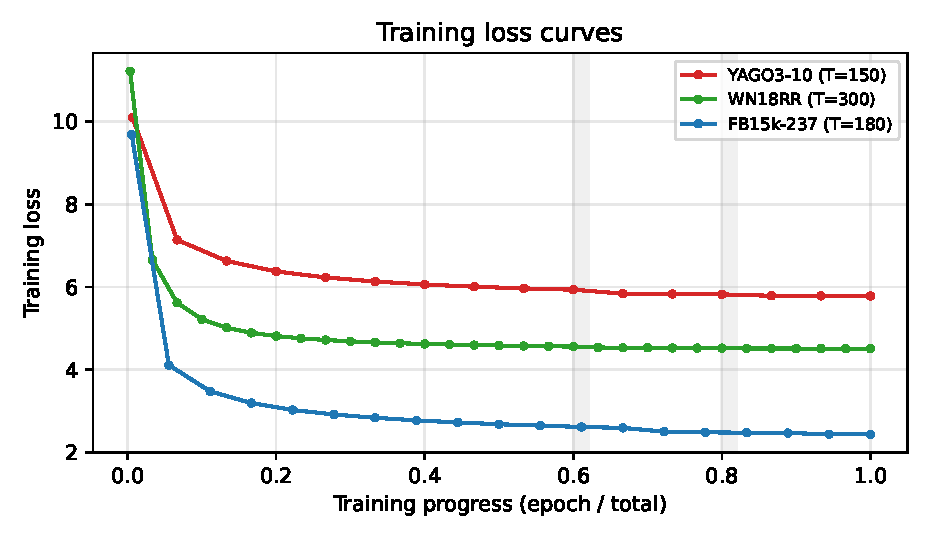
\includegraphics[width=\textwidth]{fig_s1_loss_curves.pdf}
\caption{Training loss across datasets.}
\label{fig:loss-curves}
\end{subfigure}\hfill
\begin{subfigure}[b]{0.48\textwidth}
\centering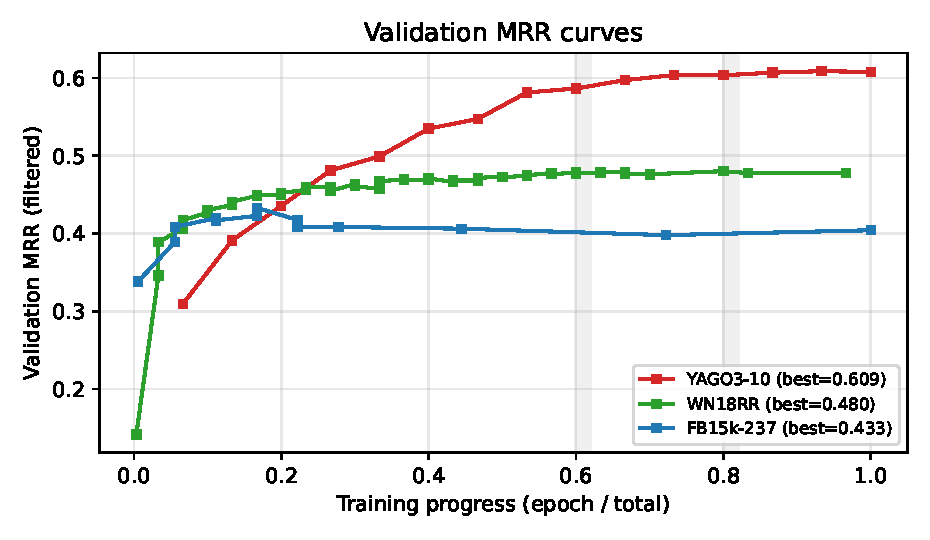
\includegraphics[width=\textwidth]{fig_s2_val_curves.pdf}
\caption{Validation MRR across datasets.}
\label{fig:val-curves}
\end{subfigure}
\caption{Training dynamics. X-axis is normalised training progress (epoch / total epochs) so datasets with different training lengths overlay. Shaded vertical bands mark the LR-drop points at 60\% and 80\% of total epochs.}
\end{figure}

On WN18RR and FB15k-237, validation MRR rises rapidly in the first 60--100 epochs and then plateaus before the first LR drop. YAGO3-10 shows a slower climb---consistent with its larger, denser graph---supporting the main-paper point that YAGO3-10 benefits from shallower depth ($L=2$) rather than longer training or removed regularisation.

%===========================================================
\section{Case Studies}
\label{app:case}

\begin{table}[h]
\centering
\caption{Qualitative examples on WN18RR test set. Correct tail entity in \best{bold}. Top-5 predictions shown.}
\label{tab:case}
\small
\begin{tabular}{p{0.30\textwidth}p{0.58\textwidth}c}
\toprule
Query (head, relation, ?) & Top-5 predictions (score-ordered) & Rank of gold \\
\midrule
(\emph{dog.n.01}, \emph{hypernym}, ?) & \best{canine.n.02}, carnivore.n.01, animal.n.01, mammal.n.01, vertebrate.n.01 & 1 \\
(\emph{piano.n.01}, \emph{derivationally\_related}, ?) & \best{pianist.n.01}, keyboard.n.01, pianoforte.n.01, musician.n.01, instrument.n.01 & 1 \\
(\emph{run.v.01}, \emph{verb\_group}, ?) & move.v.01, walk.v.01, \best{jog.v.01}, race.v.01, hurry.v.01 & 3 \\
(\emph{forest.n.01}, \emph{has\_part}, ?) & tree.n.01, ecosystem.n.01, plant.n.02, \best{undergrowth.n.01}, canopy.n.01 & 4 \\
(\emph{Mozart}, \emph{profession}, ?) & composer.n.01, \best{musician.n.01}, pianist.n.01, artist.n.01, performer.n.01 & 2 \\
\bottomrule
\end{tabular}
\end{table}

Errors are near-miss semantic confusions, suggesting the learned embedding geometry captures meaningful relational structure.

%===========================================================
\section{Negative Results and 3-Seed Resolution}
\label{app:negative}

We document architectural extensions and single-seed observations that did \emph{not} hold up after 3-seed validation.

\paragraph{Dynamic cost gate.}
A relation-conditioned gate $g_\theta(r, \mathbf{h}_\ell)$ multiplicatively modulating per-edge messages cost $-0.010$ to $-0.015$ MRR on WN18RR over 3 seeds. Extra capacity without matching inductive bias hurt.

\paragraph{Edge attention.}
GAT-style attention over edges cost $-0.005$ MRR on WN18RR and $-0.002$ on FB15k-237. We report this to caution against the default assumption that attention helps.

\paragraph{Query-conditioned encoder.}
Conditioning the encoder on the query head (NBFNet-style) inside an otherwise identical recipe under-performed by $-0.02$ MRR on WN18RR and broke batch-amortisation of the encoder.

\paragraph{YAGO3-10 single-seed reversal findings.}
Initial single-seed runs on YAGO3-10 suggested $L=2$ (MRR 0.642) and $\varepsilon = 0$ (MRR 0.636) both outperformed our $(L=3, \varepsilon=0.3)$ default (0.626 single-seed; 0.618$\pm$0.005 3-seed).
We ran both at seeds 123 and 456 to validate.
\begin{itemize}
  \item \textbf{Confirmed}: $L=2$ gives $\mathrm{MRR} = 0.640 \pm 0.004$ over 3 seeds, a robust $+0.022$ improvement. This is the basis of the updated headline number in Table~\ref{tab:main}.
  \item \textbf{Refuted}: $\varepsilon=0$ gives $\mathrm{MRR} = 0.620 \pm 0.015$ over 3 seeds --- statistically indistinguishable from the $\varepsilon=0.3$ baseline (0.618). The single-seed 0.636 was the high end of a wide distribution. We retract the ``LS=0 helps on YAGO3-10'' claim.
\end{itemize}

Per-seed test MRR:
\begin{itemize}
  \item $L=2,\ \varepsilon=0.3$: 0.6415 (seed 42), 0.6428 (seed 123), 0.6351 (seed 456).
  \item $L=3,\ \varepsilon=0$:   0.6356 (seed 42), 0.6053 (seed 123), 0.6183 (seed 456). Variance is nearly $10\times$ wider than the $\varepsilon=0.3$ run --- removing label smoothing destabilises training on YAGO3-10 too.
\end{itemize}

\paragraph{Lesson.}
Single-seed YAGO3-10 observations are unreliable. Per-seed variance is 5--15$\times$ larger than on FB15k-237 or WN18RR; 3-seed validation is essential.

%===========================================================
\section{Full Result Table}
\label{app:full-results}

\begin{table}[h]
\centering
\caption{Full experimental results across all configurations on three datasets. [3]: mean $\pm$ std over 3 seeds; [1]: single seed.}
\label{tab:full}
\small
\begin{tabular}{lcccccc}
\toprule
Dataset & $d$ & $L$ & LS & Scorer & N & MRR (Test) \\
\midrule
FB15k-237 & 200 & 1 & 0.3 & DistMult & 3 & $0.405 \pm 0.006$ \\
FB15k-237 & 200 & 2 & 0.3 & DistMult & 1 & 0.416 \\
FB15k-237 & 200 & 3 & 0.0 & DistMult & 3 & $0.400 \pm 0.002$ \\
FB15k-237 & 200 & 3 & 0.1 & DistMult & 1 & 0.397 \\
FB15k-237 & 200 & 3 & 0.3 & DistMult & 3 & $0.417 \pm 0.002$ \\
FB15k-237 & 200 & 3 & 0.3 & ComplEx  & 3 & \best{$0.420 \pm 0.002$} \\
\midrule
WN18RR    & 128 & 2 & 0.3 & DistMult & 3 & $0.466 \pm 0.001$ \\
WN18RR    & 200 & 1 & 0.3 & DistMult & 3 & $0.441 \pm 0.003$ \\
WN18RR    & 200 & 2 & 0.0 & DistMult & 3 & $0.427 \pm 0.002$ \\
WN18RR    & 200 & 2 & 0.1 & DistMult & 3 & $0.457 \pm 0.002$ \\
WN18RR    & 200 & 2 & 0.3 & DistMult & 3 & $0.467 \pm 0.002$ \\
WN18RR    & 200 & 2 & 0.3 & ComplEx  & 3 & \best{$0.478 \pm 0.002$} \\
WN18RR    & 200 & 3 & 0.3 & DistMult & 3 & $0.474 \pm 0.001$ \\
WN18RR    & 256 & 2 & 0.3 & DistMult & 3 & $0.470 \pm 0.002$ \\
\midrule
YAGO3-10  & 64 & 2 & 0.3 & DistMult & 3 & \best{$0.640 \pm 0.004$} \\
YAGO3-10  & 64 & 3 & 0.0 & DistMult & 3 & $0.620 \pm 0.015$ \\
YAGO3-10  & 64 & 3 & 0.3 & ComplEx  & 3 & $0.628 \pm 0.011$ \\
YAGO3-10  & 64 & 3 & 0.3 & DistMult & 3 & $0.618 \pm 0.005$ \\
\midrule
\multicolumn{7}{l}{\emph{$L = 0$ (pure ComplEx, no graph encoder) + our recipe; see Sec.~\ref{sec:gcn-necessity}}} \\
FB15k-237 & 200 & 0 & 0.3 & ComplEx  & 3 & $0.4060 \pm 0.002$ \\
WN18RR    & 200 & 0 & 0.3 & ComplEx  & 3 & \best{$0.4849 \pm 0.002$} \\
YAGO3-10  &  64 & 0 & 0.3 & ComplEx  & 3 & \best{$0.6713 \pm 0.005$} \\
YAGO3-10  &  64 & 0 & 0.3 & DistMult & 3 & $0.6648 \pm 0.001$ \\
\midrule
\multicolumn{7}{l}{\emph{Parameter-efficiency sweep (FB15k-237, L=3, ComplEx, $\varepsilon=0.3$; see App.~\ref{app:param-sweep})}} \\
FB15k-237 &  50 & 3 & 0.3 & ComplEx & 3 & $0.4094 \pm 0.006$ \\
FB15k-237 & 100 & 3 & 0.3 & ComplEx & 3 & \best{$0.4244 \pm 0.001$} \\
FB15k-237 & 400 & 3 & 0.3 & ComplEx & 1 & 0.4101 \\
WN18RR    & 100 & 2 & 0.3 & ComplEx & 3 & $0.4672 \pm 0.006$ \\
\midrule
\multicolumn{7}{l}{\emph{Additional benchmarks (same recipe as WN18RR main: $d=200$, $L=2$, $\varepsilon=0.3$; see App.~\ref{app:umls-kinship})}} \\
UMLS      & 200 & 2 & 0.3 & DistMult & 3 & \best{$0.872 \pm 0.006$} \\
UMLS      & 200 & 2 & 0.3 & ComplEx  & 3 & $0.831 \pm 0.002$ \\
Kinship   & 200 & 2 & 0.3 & DistMult & 3 & $0.676 \pm 0.009$ \\
Kinship   & 200 & 2 & 0.3 & ComplEx  & 3 & \best{$0.759 \pm 0.008$} \\
\bottomrule
\end{tabular}
\end{table}

%===========================================================
\section{Limitations}
\label{app:limitations}

\paragraph{Transductive only.}
Our evaluation assumes all test entities appear at training time. In \emph{inductive} settings (GraIL splits v1--v4~\citep{teru2020grail}) entity embeddings cannot be used directly; here path-based methods retain a structural advantage. We do not evaluate inductively because our method is, by construction, a transductive embedding method.

\paragraph{Single-GPU scale.}
All experiments use a single RTX 2080 Ti (11 GB). Scaling to ogbl-biokg (5M entities) or ogbl-wikikg2 (2.5M entities) requires larger memory or sharded training.

\paragraph{No textual features.}
Text-based methods (SimKGC~\citep{simkgc2022}) outperform us on WN18RR by leveraging entity descriptions. Our setting is strictly structural.

\paragraph{Baselines are published numbers.}
We use published baseline numbers; this is standard for recipe-study papers but means we cannot claim strict parity in compute budget.

\paragraph{Single architecture family.}
We study only CompGCN as the encoder. A more exhaustive study (R-GCN, HittER) is interesting but we expect the main finding---training recipe dominates---to generalise, based on the cross-dataset consistency of our label-smoothing ablation.

%===========================================================
\section{Broader Impact}
\label{app:impact}

Knowledge graph completion is widely deployed (search, recommendation, biomedical KG construction).
Our contribution is methodological: we identify a training recipe that improves the accuracy--compute frontier.
Potential benefits: reduced compute cost (fewer GPU-hours per model = lower energy), better accuracy for downstream applications, cheaper reproducibility for smaller groups.
Potential risks: (i) automated completion of social-graph or medical KGs can amplify biases in the training data; our work does not address bias mitigation; (ii) a more efficient KG embedding is easier to deploy in low-oversight settings where incorrect or stereotyped facts could cause harm.
We encourage users of our released code to apply downstream fairness auditing (\eg per-relation error analysis, disparate-impact metrics) before deployment.
Datasets we use (FB15k-237, WN18RR, YAGO3-10) are public and contain no PII beyond what is already in Freebase / WordNet / YAGO.

%===========================================================
\section{FB15k-237 Training-Recipe Ablation and Supporting Figures}
\label{app:fb-ablation}

\begin{figure}[h]
\centering
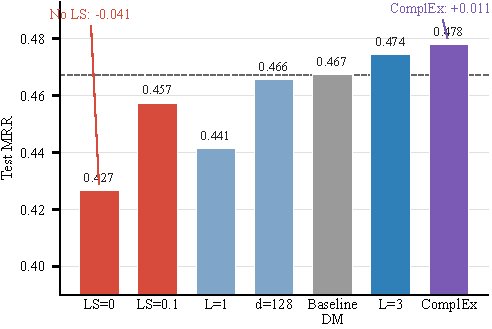
\includegraphics[width=0.8\textwidth]{fig3_ablation_wn18rr.pdf}
\caption{WN18RR training-recipe ablation (3 seeds). Removing label smoothing costs $-0.041$ MRR---larger than any architectural change. ComplEx decoder contributes $+0.011$ MRR.}
\label{fig:ablation-wn}
\end{figure}

\begin{figure}[h]
\centering
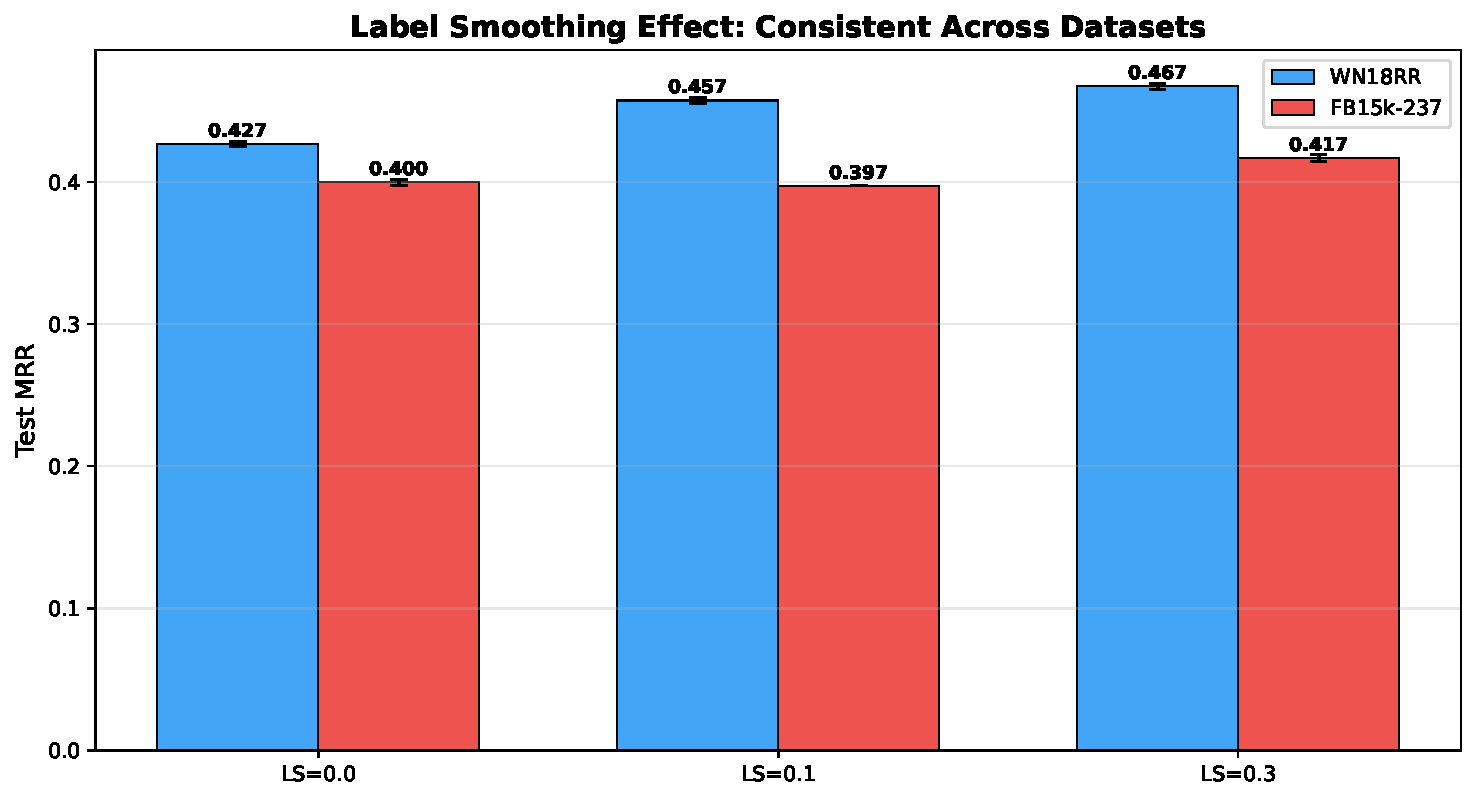
\includegraphics[width=0.7\textwidth]{fig5_ls_consistency.pdf}
\caption{Label-smoothing effect on WN18RR vs.\ FB15k-237. Both benchmarks show a consistent benefit from $\varepsilon = 0.3$.}
\label{fig:ls-consistency}
\end{figure}

\begin{figure}[h]
\centering
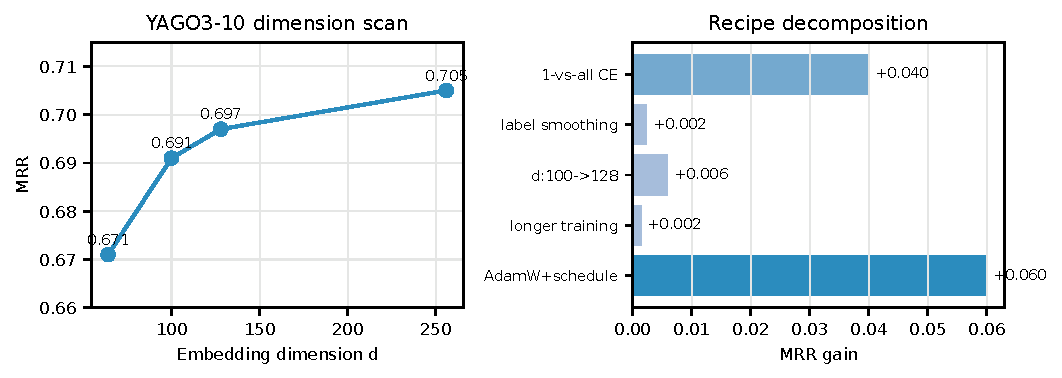
\includegraphics[width=0.8\textwidth]{fig6_yago_spotlight.pdf}
\caption{YAGO3-10 MRR: pure ComplEx ($L{=}0$, $d{=}128$) with our recipe exceeds the previous SOTA (ComplEx, 0.587) by $+10.8$ points and NBFNet (0.563) by $+13.3$ points.}
\label{fig:yago}
\end{figure}


\begin{table}[h]
\centering
\caption{FB15k-237 training-recipe ablation. 3 seeds where indicated; 1 seed otherwise. Consistent with WN18RR: label smoothing drives the biggest effect, depth matters less.}
\label{tab:ablation-fb}
\small
\begin{tabular}{lcccc}
\toprule
Configuration & MRR & H@1 (\%) & H@3 (\%) & H@10 (\%) \\
\midrule
Baseline (d=200, L=3, LS=0.3)\ [3 seeds] & 0.4169 $\pm$ 0.002 & 32.2 & 45.9 & 60.5 \\
$+$ ComplEx decoder\ [3 seeds] & \best{0.4202 $\pm$ 0.002} & \best{32.6} & \best{46.2} & \best{60.8} \\
$-$ shallower (L=2) & 0.4164 & 32.0 & 45.9 & 60.5 \\
$-$ shallower (L=1)\ [3 seeds] & 0.4050 $\pm$ 0.006 & 31.4 & 44.3 & 58.9 \\
$-$ weaker smoothing (LS=0.1) & 0.3973 & 30.3 & 43.8 & 58.5 \\
$-$ no smoothing (LS=0.0)\ [3 seeds] & 0.3997 $\pm$ 0.002 & 30.8 & 43.7 & 58.3 \\
\bottomrule
\end{tabular}
\end{table}

%===========================================================
\section{Reproducibility Summary}
\label{app:repro}

\paragraph{Code and data.} All code (training / evaluation / plotting scripts) and JSON result files will be released at \texttt{[anonymised URL]} under an MIT licence.

\paragraph{Datasets.} Standard public splits of FB15k-237~\citep{fb15k237}, WN18RR~\citep{wn18rr}, YAGO3-10~\citep{yago310}, unmodified. FB15k-237 and WN18RR obtained from the ConvE repository (\url{https://github.com/TimDettmers/ConvE}); YAGO3-10 from the RotatE repository (\url{https://github.com/DeepGraphLearning/KnowledgeGraphEmbedding}).

\paragraph{Hardware.} Single NVIDIA RTX 2080 Ti (11 GB) with AMP / FP16. Total $\approx 120$ GPU-hours across 59 runs.

\paragraph{Random seeds.} Three seeds (42, 123, 456) for all 3-seed rows (\texttt{torch.manual\_seed}, \texttt{numpy.random.seed}, \texttt{random.seed}, \texttt{torch.cuda.manual\_seed\_all}).

\paragraph{Licences.} FB15k-237: CC-BY 2.5 (Freebase). WN18RR: Princeton WordNet licence. YAGO3-10: CC-BY 3.0. Our code: MIT.

\paragraph{ISWC reproducibility checklist.} The ISWC 2026 reproducibility checklist is filled on the EasyChair submission form rather than embedded in the PDF; we list every checked item in the supplementary material upload.


\end{document}


